% Supplement to "Rotatable Networks". Compile AFTER main.tex so that
% xr can resolve cross-references into main.aux:
%   pdflatex main && bibtex main && pdflatex main && pdflatex main
%   pdflatex supplement && bibtex supplement && pdflatex supplement x2
\documentclass[12pt]{article}

\usepackage[margin=1in]{geometry}
\usepackage{amsmath,amssymb,amsthm,mathtools}
\usepackage{bm}
\usepackage{graphicx}
\usepackage{booktabs}
\usepackage[protrusion=true,expansion=false]{microtype}
\usepackage[round]{natbib}
\usepackage{setspace}
\usepackage{caption}
\usepackage{enumitem}
\usepackage{xr}
% xr imports main.aux; suppress its \bibcite lines so shared citations
% are not defined twice (they are re-defined identically by supplement.aux)
\makeatletter
\let\saved@bibcite\bibcite
\def\bibcite#1#2{}
\externaldocument{main}
\let\bibcite\saved@bibcite
\makeatother
\usepackage{xcolor}
\definecolor{linkink}{RGB}{28,60,120}
\usepackage[colorlinks=true,linkcolor=linkink,citecolor=linkink,urlcolor=linkink]{hyperref}
\captionsetup{font={small,stretch=1.05},labelfont=bf}

\doublespacing

\newtheorem{theorem}{Theorem}
\newtheorem{proposition}{Proposition}
\newtheorem{corollary}{Corollary}
\newtheorem{lemma}{Lemma}
\theoremstyle{definition}
\newtheorem{definition}{Definition}
\theoremstyle{remark}
\newtheorem{remark}{Remark}
\renewcommand{\thesection}{S\arabic{section}}
\renewcommand{\thetheorem}{S\arabic{theorem}}
\renewcommand{\theproposition}{S\arabic{proposition}}
\renewcommand{\thecorollary}{S\arabic{corollary}}
\renewcommand{\thelemma}{S\arabic{lemma}}
\renewcommand{\theremark}{S\arabic{remark}}
\renewcommand{\thetable}{S\arabic{table}}
\renewcommand{\theequation}{S\arabic{equation}}
\renewcommand{\thefigure}{S\arabic{figure}}

\newcommand{\R}{\mathbb{R}}
\newcommand{\N}{\mathbb{N}}
\newcommand{\E}{\mathbb{E}}
\newcommand{\Prob}{\mathbb{P}}
\newcommand{\OO}{\mathbb{O}}
\newcommand{\eqd}{\overset{d}{=}}
\newcommand{\tod}{\overset{d}{\to}}
\newcommand{\toas}{\overset{\mathrm{a.s.}}{\to}}
\newcommand{\toP}{\overset{P}{\to}}
\newcommand{\iid}{\overset{\mathrm{iid}}{\sim}}
\newcommand{\Sym}{\mathrm{Sym}}
\newcommand{\tr}{\operatorname{tr}}
\newcommand{\diag}{\operatorname{diag}}
\newcommand{\spec}{\operatorname{spec}}
\newcommand{\hollow}{\operatorname{hollow}}
\newcommand{\Haar}{\mathrm{Haar}}
\newcommand{\GOE}{\mathrm{GOE}}
\newcommand{\SaS}{\mathrm{S}\alpha\mathrm{S}}
\newcommand{\lam}{\lambda}
\newcommand{\blam}{\bm{\lambda}}
\newcommand{\bgam}{\bm{\gamma}}
\DeclareMathOperator*{\argmax}{arg\,max}

\title{\bfseries Supplement to ``Rotatable Networks''}

\author{Author names blinded for review}
\date{}

\begin{document}
\maketitle

This Supplement contains the formal statements deferred from the main
text (Section~S1), all proofs (Section~S2), additional experimental
details (Section~S3), and the data and computation appendix
(Section~S4). Cross-references of the form Theorem~1 or
equation~\eqref{eq:rep} point to the main text.

\section{Deferred statements}
\label{supp:statements}

This section states the results that the main text uses through pointers.
Numbering is internal to the Supplement; references such as
Theorem~\ref{thm:rep} point to the main text.



\begin{proposition}[Cycle densities are power sums]
\label{sprop:ident}
Let $X\sim P^{\mathrm{net}}_{\sigma,\blam}$ with $\sum_k\lam_k^2<\infty$.
For distinct indices $i_1,\dots,i_m$, $m\ge3$,
\begin{equation*}
\E\bigl[X_{i_1i_2}X_{i_2i_3}\cdots X_{i_mi_1}\bigr] \;=\; p_m(\blam)
\;=\;\sum_k \lam_k^m ,
\qquad
\E\bigl[X_{12}^2\bigr] \;=\; \sigma^2 + p_2(\blam).
\end{equation*}
More generally, for a finite simple graph $F$ with at least one edge:
$\E\prod_{e\in F}X_e=0$ whenever some edge of $F$ lies in no cycle of $F$
(in particular for every tree), and
$\E\prod_{e\in F}X_e=\prod_{j\le r}p_{|C_j|}(\blam)$ when $F$ is a
vertex-disjoint union of cycles $C_1,\dots,C_r$, each of length at least
three. The product formula does not extend further: two triangles sharing
one vertex have expectation $p_3(\blam)^2+2\,p_6(\blam)$, and a doubled
edge has expectation $\sigma^2+p_2(\blam)$. Consequently the noise level
and the multiset of nonzero eigenvalues, $(\sigma^2,\{\lam_k\})$, are
identified by the ergodic law, and two parameter pairs yield the same
network law if and only if they agree in this sense.
\end{proposition}

\begin{proposition}[Emergence and estimation]
\label{sprop:bbp}
Let $\sigma>0$, let $X\sim R_{0,\sigma,\blam}$ have finitely many
nonzero $\lam_1\ge\dots\ge\lam_K$ (all $\ne0$), and let
$\mu_{1}\ge\dots\ge\mu_n$ be the eigenvalues of the fully observed
corner $X_n/(\sigma\sqrt n)$; the zero-diagonal observation changes
every $\mu_j$ by $O_P(\log n/\sqrt n)$ and all statements below are
robust to it. Set $s_k=\sqrt n\,\lam_k/\sigma$. Then, as $n\to\infty$
with the array fixed:
\begin{enumerate}[label=(\roman*),itemsep=1pt,topsep=2pt]
\item (Resolution.) For every $k$ with $\lam_k>0$,
$\mu_k/s_k\toas1$ and
$\mu_k-(s_k+1/s_k)=s_k\bigl(\lVert\Xi_k\rVert^2/n-1\bigr)+o_P(1)
=O_P(1)$, the $O_P(1)$ term reflecting the realized factor norm; the
mirrored statements hold for $\lam_k<0$ at the smallest eigenvalues.
For every fixed $\varepsilon>0$, the number of eigenvalues outside
$[-2-\varepsilon,2+\varepsilon]$ converges a.s.\ to
$\#\{k:\lam_k\neq0\}$.
\item (Finite-$n$ boundary.) Against local sequences
$\lam^{(n)}=c\,n^{-1/2}$ the transition is at $c=\sigma$: for
$c<\sigma$ no eigenvalue separates from the bulk and no consistent
test exists along the contiguous sequences
\citep{onatski2013asymptotic,perry2018optimality}; for $c>\sigma$ the
top eigenvalue separates and its eigenvector correlates with the
planted factor, with squared overlap $\to 1-c^{-2}\sigma^2$.
\item (Plug-in estimation.) The empirical spectral distribution of
$X_n/\sqrt n$ converges weakly a.s.\ to the semicircle law of radius
$2\sigma$, so
$\hat\sigma=\hat q_{3/4}(\spec(X_n/\sqrt n))/q_{3/4}^{\rm sc}$,
$q_{3/4}^{\rm sc}\approx0.8079$, satisfies $\hat\sigma\toas\sigma$.
For each $j$ with $|\mu_j|>2+\varepsilon_n$ set
$\hat\lam_j=\operatorname{sgn}(\mu_j)\,
\tfrac{\hat\sigma}{\sqrt n}\,\hat s_j$ with
$\hat s_j=\bigl(|\mu_j|+\sqrt{\mu_j^2-4}\bigr)/2$; then
$\hat\lam_k/\lam_k\toas1$ for every $k$ with $\lam_k\ne0$, and, with
$\varepsilon_n\downarrow0$ satisfying
$n^{2/3}\varepsilon_n\to\infty$ and
$\varepsilon_n\sqrt n/\log n\to\infty$,
$\hat K=\#\{j:|\mu_j|>2+\varepsilon_n\}$ is a consistent estimator of
the number of spikes.
\end{enumerate}
\end{proposition}

\begin{corollary}[Non-spectral summaries are conditionally parameter-free]
\label{scor:ancillary}
Let $S:\Sym_n\to\R^q$ be any measurable network statistic. Under any
family $\mathcal{P}$ of orthogonally invariant laws:
(i) the conditional law of $S(X)$ given $D(X)$ is parameter-free and
exactly simulable by Haar rotation of the observed spectrum;
(ii) $\E[S(X)\mid D]$ is a spectral statistic, and for any parameter
$\theta$ of any subfamily, any estimator or test based on $S$ is weakly
dominated by one based on $D$ alone (Rao--Blackwell; convex losses,
tests via the conditional test function);
(iii) on the simple-spectrum event, any statistic of the frame $V(X)$
alone is ancillary: $V(X)\sim\nu_n$, the sign-normalized Haar law of
Theorem~\ref{thm:suff}(iii), whose distribution is free of the
parameter.
\end{corollary}

\begin{proposition}[Consistency against localized spikes]
\label{sprop:consistency}
Let $X^{(n)}$ follow the spiked model
$X^{(n)}=\tfrac{\sigma}{\sqrt n}W_n+\theta v_nv_n^\top$ with $\theta>\sigma$
and unit vectors $v_n$ satisfying
$\liminf_n \lVert v_n\rVert_4^4 \ge c_0>0$
(e.g.\ $v_n$ supported on $O(1)$ many coordinates, or any hub-like
direction). Let $p^{(n)}$ be the conditional $p$-value of
$T_{\mathrm{IPR}}$ with $B_n\to\infty$. Then $p^{(n)}\toP0$; the test is
consistent. Under the rotatable null with the same spectrum,
$T_{\mathrm{IPR}}=O_P(\log n/n)$, so the separation is by a factor of
order $n/\log n$.
\end{proposition}

\begin{corollary}[Spherical spikes are null; localized detection threshold]
\label{scor:boundary}
Fix $\sigma>0$.
(i) If $v$ is uniform on the unit sphere, independent of $W_n$, then
$\sigma W_n/\sqrt n+\theta vv^\top$ is orthogonally invariant for
every $\theta$, hence lies in the composite null of
Theorem~\ref{thm:test}; the conditional test has exact level against
it at every spike strength.
(ii) For $\ell_4$-nondegenerate directions
($\liminf\lVert v_n\rVert_4^4\ge c_0>0$) and every fixed
$s=\theta/\sigma>1$, the IPR test is consistent
(Proposition~\ref{sprop:consistency}).
(iii) For every fixed $s<1$ with spherical direction, the alternatives
are contiguous to the point null with $\sigma$ fixed and $\blam=0$
\citep{perry2018optimality}; every test sequence whose size tends to
zero has power tending to zero, so no consistent test exists.
Sparse priors can admit sub-boundary consistent detection by
exhaustive scans outside this battery, and positive-size tests below
the boundary may retain nontrivial power, which contiguity does not
exclude.
\end{corollary}

\begin{remark}[Hollow laws and Haar orbits are mutually singular]
\label{srem:hollowtv}
The requirement that the diagonal be retained is essential. Suppose
that \(Y\in\Sym_n\) is invariant under orthogonal conjugation and is
hollow almost surely. For every deterministic unit vector
\(a\in\mathbb R^n\), choose \(q_a\in\OO(n)\) such that
\(q_a^\top e_1=a\). Orthogonal invariance gives
\[
a^\top Ya
=
e_1^\top q_aYq_a^\top e_1
\eqd
e_1^\top Ye_1
=
0.
\]
Let \(\mathcal A\) be a countable dense subset of the unit sphere.
With probability one,
\[
a^\top Ya=0
\qquad\text{for every }a\in\mathcal A.
\]
For each realization in this probability-one event, continuity of
\(a\mapsto a^\top Ya\) extends the equality to the entire unit sphere,
and homogeneity extends it to all \(a\in\mathbb R^n\). Since a real
symmetric matrix is determined by its quadratic form, \(Y=0\) almost
surely.
Thus no nondegenerate hollow law, including a nondegenerate
zero-completed network law
\(P^{\mathrm{net}}_{\sigma,\blam}\), can be exactly invariant under
all orthogonal conjugations. Theorem~\ref{thm:suff} applies exactly to
the corresponding fully observed symmetric corner before hollowing.
There is also a stronger obstruction in total variation. Let
\[
\mathcal H_n
:=
\left\{
x\in\Sym_n:
x_{11}=\cdots=x_{nn}=0
\right\}.
\]
For every \(d\in\Delta_n\setminus\{0\}\),
\[
\kappa(d,\mathcal H_n)=0.
\]
For \(n=1\), this is immediate. For \(n\geq2\), if
\(U\sim\Haar_n\), then its first row is uniformly distributed on the
unit sphere and
\[
\left(U\diag(d)U^\top\right)_{11}
=
\sum_{i=1}^n d_iU_{1i}^2.
\]
As a function of the first row of \(U\), this is a nonzero
real-analytic function on the unit sphere. Its zero set has Haar
surface measure zero. Hence the Haar orbit belongs to
\(\mathcal H_n\) with probability zero.
In contrast, suppose that \(X\) is hollow almost surely and let
\(Q(d,\cdot)\) be a regular conditional law of \(X\) given
\(D(X)=d\). Then
\[
Q(d,\mathcal H_n)=1
\qquad
\text{for \(P_D\)-almost every }d.
\]
Under the convention
\[
d_{\mathrm{TV}}(\mu,\eta)
:=
\sup_{A\in\mathcal B(\Sym_n)}
|\mu(A)-\eta(A)|,
\]
it follows that
\[
d_{\mathrm{TV}}\!\left(
Q(d,\cdot),\kappa(d,\cdot)
\right)
=
1
\qquad
\text{for \(P_D\)-almost every }d\neq0.
\]
Therefore an exactly hollow nonzero observation cannot satisfy a
nontrivial conditional total-variation approximation to the Haar
orbit. Any useful approximation must use a weaker metric, a diagonal
augmentation model, or a different observation model.
\end{remark}

\begin{remark}[Fixed-diagonal observations]
\label{srem:fixeddiag}
The conclusion is nontrivial only when \(\varepsilon<1\). Fix
\(c\in\mathbb R\), and define
\[
\mathcal H_{n,c}
:=
\left\{
x\in\Sym_n:
x_{11}=\cdots=x_{nn}=c
\right\}.
\]
If \(P(\mathcal H_{n,c})=1\), then
\[
P_d(\mathcal H_{n,c})=1
\qquad
\text{for \(P_D\)-almost every \(d\)}.
\]
On the other hand, if \(d\neq c\mathbf 1_n\), then
\[
\kappa_d(\mathcal H_{n,c})=0.
\]
Indeed, if \(V\) is the first row of a Haar-distributed orthogonal
matrix, then \(V\) is uniform on the unit sphere and
\[
\left(U\diag(d)U^\top\right)_{11}
=
\sum_{i=1}^{n}d_iV_i^2.
\]
On the unit sphere, the equality
\[
\sum_{i=1}^{n}d_iV_i^2=c
\]
is equivalent to
\[
\sum_{i=1}^{n}(d_i-c)V_i^2=0.
\]
If the restriction of this polynomial to the sphere were identically
zero, evaluation at the coordinate vectors would give
\(d_i=c\) for every \(i\). Thus, when \(d\neq c\mathbf 1_n\), it is a
nonzero real-analytic function on the sphere. For \(n\geq2\), its zero
set has surface measure zero; the case \(n=1\) is immediate.
Therefore
\[
d_{\mathrm{TV}}(P_d,\kappa_d)=1
\qquad
\text{for \(P_D\)-almost every }
d\in\Delta_n\setminus\{c\mathbf 1_n\}.
\]
Consequently, if \(P(\mathcal H_{n,c})=1\) and
\eqref{eq:approx-haar-conditionals} holds with \(\varepsilon<1\), then
\[
P_D\{c\mathbf 1_n\}=1.
\]
Every real symmetric matrix whose eigenvalues all equal \(c\) is
\(cI_n\), so
\[
P\{cI_n\}=1.
\]
Thus the full-TV assumption cannot yield a nontrivial guarantee for
an intrinsically hollow nonzero matrix or for a nonidentity
correlation matrix with fixed unit diagonal. Common preprocessing is
permitted only after beginning with an unprocessed matrix satisfying
\eqref{eq:approx-haar-conditionals}; preprocessing cannot itself make
an intrinsically fixed-diagonal observation satisfy that assumption.
\end{remark}

\section{Proofs}
\label{supp:proofs}

Throughout the appendix, $\Haar_n$ denotes Haar probability measure on
$\OO(n)$, and ``ergodic'' means extreme in the convex set of jointly
rotatable laws.

\subsection{Proof of Theorem~\ref{thm:rep}}

\emph{Parameter space.}
\paragraph{Canonical parameter convention.}
For \(a,b\in\mathbb R\), write \(a\succeq_*b\) if
\[
|a|>|b|
\quad\text{or}\quad
\bigl(|a|=|b|\text{ and }a\geq b\bigr),
\]
and define
\[
\ell_{2,*}
:=
\left\{
\blam=(\lam_k)_{k\geq1}\in\ell_2:
\lam_k\succeq_*\lam_{k+1}
\text{ for every }k
\right\}.
\]
Give \(\ell_{2,*}\) the Borel \(\sigma\)-field inherited from the
norm topology of \(\ell_2\). It is a Borel subset of \(\ell_2\), and
it contains exactly one ordered representative of each signed
multiset of nonzero square-summable coefficients; if the multiset is
finite, append zeros. Set
\[
\Theta
:=
\mathbb R\times[0,\infty)\times\ell_{2,*},
\]
with its product Borel \(\sigma\)-field.

\begin{proof}
The relation \(\succeq_*\) is Borel on \(\mathbb R^2\), and therefore
\(\ell_{2,*}\) is a Borel subset of \(\ell_2\). Every
\(\ell_2\)-sequence has only finitely many coordinates of magnitude
exceeding any fixed positive number, and its coordinates tend to
zero. Every nonempty remaining collection of nonzero coordinates has
a largest element under \(\succeq_*\): its positive supremal
magnitude is attained because only finitely many coordinates can
exceed half that supremum. Consequently, every signed multiset of
nonzero square-summable coordinates admits exactly one ordering by
\(\succeq_*\), with zeros appended in the finite case. Thus
\(\Theta\) is a standard Borel space.
We next establish convergence and measurability. Fix \(i,j\) and put
\[
Z_{k,ij}
:=
\lam_k\bigl(\xi_{ki}\xi_{kj}-\delta_{ij}\bigr).
\]
For fixed \(\theta\), the variables \((Z_{k,ij})_{k\geq1}\) are
independent and centered, and
\[
\sum_{k=1}^{\infty}\mathbb E Z_{k,ij}^2
=
(1+\delta_{ij})
\sum_{k=1}^{\infty}\lam_k^2
<\infty.
\]
The partial sums therefore converge almost surely and in \(L^2\).
Since \(\mathbb N^2\) is countable, the convergence holds
simultaneously for all coordinates on an event of probability one.
To verify the kernel assertion, realize \(W\) and \(\xi\) on one
standard product probability space
\((\Omega,\mathcal F,\mathbb P)\), and let
\(S_m(\theta,\omega)\) be the array obtained by truncating
\eqref{eq:rep} after \(m\) spike terms. Every coordinate of \(S_m\)
is jointly Borel in \((\theta,\omega)\). The set
\[
C
:=
\bigcap_{i,j\geq1}
\left\{
(\theta,\omega):
\bigl(S_{m,ij}(\theta,\omega)\bigr)_{m\geq1}
\text{ converges}
\right\}
\]
is Borel, by the Cauchy criterion. Define \(F(\theta,\omega)\) as the
coordinatewise limit on \(C\), and as the zero array on \(C^c\).
Then \(F\) is jointly Borel and, writing
\(C_\theta:=\{\omega:(\theta,\omega)\in C\}\),
\[
\mathbb P(C_\theta)=1
\qquad\text{for every }\theta.
\]
Consequently,
\[
R_\theta
=
\mathbb P\circ F(\theta,\cdot)^{-1}.
\]
For every Borel \(B\subseteq\Sym_\infty\), the map
\(\theta\mapsto\int \mathbf 1_B(F(\theta,\omega))\,\mathbb P(d\omega)\)
is Borel. Hence \(\theta\mapsto R_\theta\) is a Borel probability
kernel.
For later use, associate with
\(\theta=(\rho,\sigma,\blam)\) the finite Borel measure
\[
m_\theta
:=
\sigma^2\delta_0
+\sum_{k\geq1}\lam_k^2\delta_{\lam_k},
\]
and define
\[
\Phi:
\Theta
\longrightarrow
\mathbb R\times\mathcal M_f(\mathbb R),
\qquad
\Phi(\theta):=(\rho,m_\theta),
\]
where \(\mathcal M_f(\mathbb R)\) is the space of finite Borel
measures on \(\mathbb R\), equipped with its weak Borel
\(\sigma\)-field. The map \(\Phi\) is Borel. Indeed, for every
bounded continuous \(f\),
\[
\int f\,dm_\theta
=
\sigma^2f(0)
+\sum_{k\geq1}\lam_k^2f(\lam_k)
\]
is the pointwise limit of Borel finite sums, and these evaluation
maps generate the weak Borel \(\sigma\)-field. The map \(\Phi\) is
also injective. Indeed,
\[
m_\theta(\{0\})=\sigma^2,
\]
and, for \(x\neq0\),
\[
\frac{m_\theta(\{x\})}{x^2}
\]
is exactly the multiplicity of the coefficient \(x\). Since
\(\Theta\) and
\(\mathbb R\times\mathcal M_f(\mathbb R)\) are standard Borel
spaces, the Lusin--Souslin theorem implies that
\(\Phi(\Theta)\) is Borel and that \(\Phi^{-1}\) is Borel on
\(\Phi(\Theta)\).
Suppose now that \(X\) is jointly rotatable. The symmetric
specialization of Kallenberg's representation theorem
\citep[Theorem~5.1 and equations~(17)--(18)]{kallenberg1988some} yields
random coefficients \(\rho\), \(a\), and
\((\alpha_k)_{k\geq1}\), independent of the Gaussian arrays, such
that
\[
\sum_{k\geq1}\alpha_k^2<\infty
\qquad\text{almost surely},
\]
and, on a suitable extension of the probability space,
\begin{equation}
\label{eq:kallenberg-symmetric}
X_{ij}
=
\rho\delta_{ij}
+a(\zeta_{ij}+\zeta_{ji})
+\sum_{k\geq1}
\alpha_k\bigl(\xi_{ki}\xi_{kj}-\delta_{ij}\bigr)
\qquad\text{almost surely},
\end{equation}
where \((\zeta_{ij})_{i,j\geq1}\) and
\((\xi_{ki})_{k,i\geq1}\) are independent arrays of i.i.d.\
\(N(0,1)\) variables.
In this normalization, Kallenberg's directing measure is
\[
\eta
:=
2a^2\delta_0
+\sum_{k\geq1}\alpha_k^2\delta_{\alpha_k}.
\]
Almost surely,
\[
(\rho,\eta)\in\Phi(\Theta),
\]
and, after an immaterial modification on a null set, we may define
\[
\theta
:=
\Phi^{-1}(\rho,\eta)
=
(\rho,\sigma,\blam).
\]
Thus
\[
\sigma=\sqrt2\,|a|,
\]
and \(\blam\) is the canonical ordering of the signed multiset of
the nonzero \(\alpha_k\)'s.
Put
\[
G_{ij}
:=
\frac{\zeta_{ij}+\zeta_{ji}}{\sqrt2},
\qquad
\varsigma(a)
:=
\begin{cases}
1,&a\geq0,\\
-1,&a<0,
\end{cases}
\qquad
W':=\varsigma(a)G.
\]
The array \(G\) has the GOE law specified above. Since this law is
symmetric under multiplication of the whole array by \(-1\), the
conditional law of \(W'\), given the directing coefficients, is the
same fixed GOE law. Hence \(W'\) is independent of the directing
coefficients and of the factor array. Moreover,
\[
a(\zeta_{ij}+\zeta_{ji})
=
\sigma W'_{ij}.
\]
Let
\[
\mathcal D
:=
\sigma\bigl(\rho,a,(\alpha_k)_{k\geq1}\bigr).
\]
Conditional on \(\mathcal D\), the Gaussian factor rows are i.i.d.
The zero coefficients may be deleted and the remaining rows may be
relabelled according to the canonical ordering; the selected rows
remain conditionally i.i.d. For any finite collection of coordinates,
this relabelling preserves the laws of the finite partial sums; the
corresponding infinite sums have the same laws by their \(L^2\)
convergence. Therefore
\[
\mathcal L(X\mid\mathcal D)
=
R_\theta
\qquad\text{almost surely}.
\]
Since \(\theta\) is \(\mathcal D\)-measurable and the right-hand side
is a Borel function of \(\theta\), the tower property gives
\[
\mathcal L(X\mid\theta)
=
R_\theta
\qquad\text{almost surely}.
\]
Therefore, if \(\Pi=\mathcal L(\theta)\), then for every Borel
\(B\subseteq\Sym_\infty\),
\[
\mathbb P\{X\in B\}
=
\mathbb E\bigl[R_\theta(B)\bigr]
=
\int_\Theta R_\vartheta(B)\,\Pi(d\vartheta).
\]
This proves \textup{(ii)}.
We next prove uniqueness of the mixing measure. Realize any mixture
with parameter law \(\Pi\) on the product construction, taking the
parameter independent of the Gaussian arrays, so that
\[
\theta\sim\Pi,
\qquad
X\mid\theta\sim R_\theta.
\]
This is a Kallenberg representation whose directing pair is
\(\Phi(\theta)=(\rho,m_\theta)\), and hence that pair has law
\(\Phi_\#\Pi\). The uniqueness and measurability assertions in
\citep[Theorem~5.1]{kallenberg1988some} imply that the law of the
directing pair is determined uniquely by the law of \(X\). Hence, if
\(\Pi\) and \(\widetilde\Pi\) generate the same array law, then
\[
\Phi_\#\Pi
=
\Phi_\#\widetilde\Pi.
\]
Applying the Borel inverse \(\Phi^{-1}\) gives
\[
\Pi=\widetilde\Pi.
\]
Thus the mixing measure is uniquely determined by the law of \(X\).
Conversely, fix \(\theta\). The centered Gaussian array \(W\) has
covariance
\[
\operatorname{Cov}(W_{ij},W_{rs})
=
\delta_{ir}\delta_{js}
+\delta_{is}\delta_{jr}.
\]
The covariance is preserved by simultaneous finitary orthogonal
conjugation. Since a centered Gaussian law is determined by its
covariance,
\[
UWU^\top\overset{d}=W
\qquad\text{for every }U\in\OO_{\mathrm{fin}}.
\]
For each \(k\), the coordinatewise-defined Gaussian sequence
\(U\xi_k\) is again a sequence of i.i.d.\ \(N(0,1)\) variables, and
all independence relations are preserved. Only finite sums are used
here; no \(\ell_2\)-valued interpretation of \(\xi_k\) is needed.
Also,
\[
UIU^\top=I.
\]
Hence every finite spike truncation of \eqref{eq:rep} is jointly
rotatable. The truncations converge coordinatewise in \(L^2\), and
conjugation by a finitary \(U\) uses only finitely many coordinates
in each entry. Passing to finite-dimensional distributions shows that
\(R_\theta\) is jointly rotatable. Since
\(\theta\mapsto R_\theta\) is a Borel kernel, every mixture of these
laws is jointly rotatable. This proves \textup{(i)}.
We next identify the ergodic laws. Suppose that, for some
\(t\in(0,1)\),
\[
R_\theta
=
tP_1+(1-t)P_2,
\]
where \(P_1\) and \(P_2\) are jointly rotatable, and let
\(\Pi_1\) and \(\Pi_2\) be their respective mixing measures. Then
\[
t\Pi_1+(1-t)\Pi_2
\]
is a mixing measure for \(R_\theta\). Uniqueness therefore gives
\[
\delta_\theta
=
t\Pi_1+(1-t)\Pi_2,
\]
which forces
\[
\Pi_1=\Pi_2=\delta_\theta
\]
and hence
\[
P_1=P_2=R_\theta.
\]
Thus \(R_\theta\) is extreme, equivalently ergodic, among the jointly
rotatable laws.
Conversely, let a jointly rotatable law \(P\) have mixing measure
\(\Pi\). If \(\Pi\) is not a point mass, then, because \(\Theta\) is
standard Borel, there is a Borel set \(A\subseteq\Theta\) with
\[
0<\Pi(A)<1.
\]
Define
\[
P_A
:=
\frac{1}{\Pi(A)}
\int_A R_\theta\,\Pi(d\theta),
\qquad
P_{A^c}
:=
\frac{1}{\Pi(A^c)}
\int_{A^c}R_\theta\,\Pi(d\theta).
\]
Then
\[
P
=
\Pi(A)P_A+\Pi(A^c)P_{A^c}.
\]
Both component laws are jointly rotatable, and they are distinct by
uniqueness of their mutually singular mixing measures. Hence \(P\)
is not extreme and therefore not ergodic. The ergodic jointly
rotatable laws are exactly the \(R_\theta\)'s.
It remains to prove the finite-dimensional assertion. Suppose that
\(\{P_n\}_{n\geq1}\) is orthogonally invariant and
sampling-consistent. The identities
\[
c_{\ell,n}
=
c_{m,n}\circ c_{\ell,m}
\qquad(\ell\geq m\geq n)
\]
make \(\{P_n\}\) a projective family. Identifying
\(\Sym_\infty\) with the product over the coordinates \((i,j)\) with
\(i\leq j\), the Daniell--Kolmogorov theorem gives a unique
probability law \(P\) on \(\Sym_\infty\) satisfying
\[
(q_n)_\#P=P_n
\qquad(n\geq1).
\]
Let \(U\in\OO_{\mathrm{fin}}\), and choose \(r\) such that
\[
U=U_r\oplus I,
\qquad
U_r\in\OO(r).
\]
For every \(m\geq r\),
\[
q_m(UXU^\top)
=
(U_r\oplus I_{m-r})
q_m(X)
(U_r\oplus I_{m-r})^\top
\overset{d}=q_m(X),
\]
where the last equality follows from the orthogonal invariance of
\(P_m\). Since leading-corner cylinders generate the product
\(\sigma\)-field,
\[
UXU^\top\overset{d}=X.
\]
Thus \(P\) is jointly rotatable, and the infinite-dimensional
representation gives one measure \(\Pi\) such that
\[
P_n
=
(q_n)_\#P
=
\int_\Theta R_\theta^{(n)}\,\Pi(d\theta)
\qquad(n\geq1).
\]
Conversely, suppose that a common \(\Pi\) gives the last display for
all \(n\). Then
\[
P
:=
\int_\Theta R_\theta\,\Pi(d\theta)
\]
is jointly rotatable and has corner laws \(P_n\). If
\(Q\in\OO(n)\), invariance of \(P\) under \(Q\oplus I\) gives
\[
Qq_n(X)Q^\top
\overset{d}
=
q_n(X),
\]
so \(P_n\) is orthogonally invariant. Moreover,
\[
c_{m,n}\circ q_m=q_n
\qquad(m\geq n),
\]
and therefore
\[
(c_{m,n})_\#P_m=P_n.
\]
Thus the family is sampling-consistent.
Finally, if both \(\Pi\) and \(\Pi'\) work for every \(n\), their
infinite mixtures have the same leading-corner laws for every \(n\),
and hence the same law on \(\Sym_\infty\). Uniqueness of the
infinite-dimensional mixing measure then gives
\[
\Pi=\Pi'.
\]
\end{proof}

\subsection{Proof of Proposition~\ref{sprop:ident}}

All expectations below are under the ergodic law with
parameters $(\sigma,\blam)$, $\rho=0$, and indices below are distinct.
Write $X_{ij}=\sigma W_{ij}+S_{ij}$, $S_{ij}=\sum_k\lam_k\xi_{ki}\xi_{kj}$
($i\neq j$); all series converge in every $L^m$, $m<\infty$ (Gaussian
chaos of order 2 with $\ell_2$ coefficients; hypercontractivity), which
justifies the moment interchanges below.

\emph{Second moments.} $\E X_{12}^2=\sigma^2+\sum_k\lam_k^2
\E[\xi^2]\E[\xi^2]=\sigma^2+p_2(\blam)$, using orthogonality of
$\{\xi_{k1}\xi_{k2}\}_k$.

\emph{Cycles.} For $m\ge3$, expand
$\E\prod_{t=1}^m X_{i_ti_{t+1}}$ (indices mod $m$). Any term containing at
least one noise factor $W_{i_ti_{t+1}}$ vanishes: $W$ is centered,
independent of $S$, and the $m$ edges of a cycle are distinct pairs, so
each $W_e$ appears at most once. For the pure factor term,
\[
\E\prod_{t=1}^m S_{i_ti_{t+1}}
=\sum_{k_1,\dots,k_m}\lam_{k_1}\cdots\lam_{k_m}\,
\E\prod_{t=1}^m \xi_{k_t i_t}\xi_{k_t i_{t+1}}
=\sum_{k_1,\dots,k_m}\prod_t\lam_{k_t}\prod_{t=1}^m
\E\bigl[\xi_{k_{t-1} i_t}\xi_{k_t i_t}\bigr],
\]
by independence across the distinct node indices $i_t$. Each node factor
$\E[\xi_{k_{t-1}i_t}\xi_{k_ti_t}]=\delta_{k_{t-1}k_t}$, so the sum
collapses to the diagonal $k_1=\dots=k_m$, giving $p_m(\blam)$. (When some
$k$'s coincide, node factors are $\E[\xi^2]=1$; no higher moments arise
because each node hosts exactly two factor variables.)

\emph{General $F$.} Let $F$ be a finite simple graph (no parallel
edges), so all edges are distinct pairs and, as in the cycle case, every
term containing a noise factor vanishes. Expanding the pure factor term
assigns a factor index $k_e$ to each edge, and independence across nodes
factorizes the expectation as
$\prod_v\E\bigl[\prod_{e\ni v}\xi_{k_e,v}\bigr]$. By Wick's rule a
node factor is nonzero only if, at that node, every index value appears
an even number of times among the incident edges; hence a term survives
only if, for every $k$, the edge set $E_k=\{e:k_e=k\}$ has even degree
at every vertex, i.e.\ is a disjoint union of cycles of $F$. If some
edge of $F$ lies in no cycle, no such assignment exists and the
expectation is zero; this covers all trees with at least one edge. If
$F$ is a vertex-disjoint union of cycles $C_1,\dots,C_r$, the even
subgraphs are exactly the unions of whole cycles, so each cycle carries
one constant index, distinct cycles share no node, every node factor is
$\E[\xi^2]=1$, and the sum over the $r$ free indices gives
$\prod_{j\le r}p_{|C_j|}(\blam)$. The restriction to vertex-disjoint
cycles is necessary: two triangles sharing a single vertex give
$p_3(\blam)^2+2\,p_6(\blam)$, because the shared node contributes
$\E[\xi^4]=3$ when the two cycles carry the same index, and a doubled
edge gives the second-moment identity $\sigma^2+p_2(\blam)$, which
includes the noise.

\emph{Identifiability.} The numbers $\{p_m(\blam)\}_{m\ge2}$ determine the
multiset $\{\lam_k\ne0\}$: power sums determine elementary symmetric
polynomials of any finite leading subset (Newton's identities), and
$p_2<\infty$ makes the point measure $\sum_k\delta_{\lam_k}$ (on
$\R\setminus\{0\}$) determined by its integrals against $x^m$, $m \ge 2$,
by a standard moment/compactness argument on the bounded support
$[-\lVert\blam\rVert_\infty,\lVert\blam\rVert_\infty]$. Then $\sigma^2=\E
X_{12}^2-p_2$. Finally, empirical cycle averages over the growing corner
converge a.s.\ to these moments (they are reverse-martingales under the
exchangeability inherited from rotatability; \citealp[Ch.~1]
{kallenberg2005probabilistic}), so the parameters are tail-measurable
functionals of $X$: distinct parameters give mutually singular ergodic
laws, proving both identifiability and the extremality claims used in
Theorem~\ref{thm:rep}. \qed

\subsection{Proof of Theorem~\ref{thm:suff}}

\emph{Conventions and the measurable eigenframe.}
\paragraph{Spectral, sufficiency, and eigenframe conventions.}
Fix \(n\geq1\). For a topological space \(E\), write
\(\mathcal B(E)\) for its Borel sigma-field, and let \(\Haar_n\)
denote normalized Haar probability measure on \(\OO(n)\). Define
\[
\Delta_n
:=
\left\{
d=(d_1,\ldots,d_n)\in\mathbb R^n:
d_1\geq\cdots\geq d_n
\right\},
\]
and
\[
\Delta_n^\circ
:=
\left\{
d\in\Delta_n:
d_i>d_{i+1}
\text{ for every }i=1,\ldots,n-1
\right\}.
\]
When \(n=1\), the last condition is vacuous, so
\(\Delta_1^\circ=\Delta_1\).
For \(x\in\Sym_n\), let
\[
D(x)
=
\bigl(D_1(x),\ldots,D_n(x)\bigr)
\in\Delta_n
\]
denote its ordered eigenvalue vector. The map
\(D:\Sym_n\to\Delta_n\) is continuous. Define
\[
\mathcal S_n
:=
D^{-1}(\Delta_n^\circ)
=
\left\{
x\in\Sym_n:
D_i(x)>D_{i+1}(x)
\text{ for }i=1,\ldots,n-1
\right\}.
\]
Thus \(\mathcal S_n\) is the Borel set of matrices having simple
spectrum.
For \(d\in\Delta_n\) and \(A\in\mathcal B(\Sym_n)\), define the
Haar-orbit kernel
\[
\kappa(d,A)
:=
\int_{\OO(n)}
\mathbf 1_A\!\left(
u\diag(d)u^\top
\right)\,\Haar_n(\mathrm{d}u).
\]
For every fixed \(d\), the map \(A\mapsto\kappa(d,A)\) is a
probability measure. Since
\[
(u,d)\longmapsto u\diag(d)u^\top
\]
is continuous, parameterized integration shows that
\(d\mapsto\kappa(d,A)\) is Borel measurable for every
\(A\in\mathcal B(\Sym_n)\). Hence \(\kappa\) is a Borel Markov
kernel from \(\Delta_n\) to \(\Sym_n\). Write \(\kappa_d:=\kappa(d,\cdot)\). Moreover, for every
\(C\in\mathcal B(\Delta_n)\),
\[
\kappa\bigl(d,D^{-1}(C)\bigr)
=
\mathbf 1_C(d).
\]
Thus \(\kappa(d,\cdot)\) is supported on the spectral fiber
\(D^{-1}(\{d\})\).
For a unit vector \(v\in\mathbb R^n\), define
\[
j(v)
:=
\min\left\{
r\in\{1,\ldots,n\}:
|v_r|
=
\max_{1\leq s\leq n}|v_s|
\right\},
\]
and
\[
s(v)
:=
\operatorname{sgn}\!\bigl(v_{j(v)}\bigr)v.
\]
The selected coordinate is nonzero, so \(s(v)\) is well defined.
For \(u=(u_1,\ldots,u_n)\in\OO(n)\), where \(u_i\) denotes the
\(i\)-th column, define
\[
\mathcal N(u)
:=
\bigl(s(u_1),\ldots,s(u_n)\bigr),
\qquad
\nu_n
:=
\Haar_n\circ\mathcal N^{-1}.
\]
The map \(\mathcal N:\OO(n)\to\OO(n)\) is Borel and is unchanged by
independent sign changes of the columns. Thus \(\nu_n\) is the
sign-normalized Haar law. In general, \(\nu_n\) is not Haar measure
on \(\OO(n)\).
We next construct a measurable ordered eigenframe. For
\(x\in\mathcal S_n\) and \(i\in\{1,\ldots,n\}\), define
\[
\Pi_i(x)
:=
\prod_{\substack{1\leq\ell\leq n\\ \ell\neq i}}
\frac{x-D_\ell(x)I_n}{D_i(x)-D_\ell(x)},
\]
where an empty product is interpreted as \(I_n\). The factors commute
because they are polynomials in \(x\). By the spectral theorem,
\(\Pi_i(x)\) is the rank-one orthogonal projection onto the eigenspace
associated with \(D_i(x)\).
Set
\[
g_{ir}(x)
:=
e_r^\top\Pi_i(x)e_r,
\qquad r=1,\ldots,n,
\]
and define
\[
r_i(x)
:=
\min\left\{
r\in\{1,\ldots,n\}:
g_{ir}(x)=\max_{1\leq s\leq n}g_{is}(x)
\right\}.
\]
For each \(r\in\{1,\ldots,n\}\),
\[
\begin{aligned}
\{x\in\mathcal S_n:r_i(x)=r\}
&=
\bigcap_{t<r}
\{x\in\mathcal S_n:g_{ir}(x)>g_{it}(x)\} \\
&\quad\cap
\bigcap_{t>r}
\{x\in\mathcal S_n:g_{ir}(x)\geq g_{it}(x)\}.
\end{aligned}
\]
Since each \(g_{ir}\) is continuous on \(\mathcal S_n\), the map
\(r_i:\mathcal S_n\to\{1,\ldots,n\}\) is Borel measurable.
Define
\[
v_i(x)
:=
\frac{\Pi_i(x)e_{r_i(x)}}
{\sqrt{
e_{r_i(x)}^\top\Pi_i(x)e_{r_i(x)}
}}.
\]
Since \(\Pi_i(x)\) is a rank-one orthogonal projection with trace one,
\[
e_{r_i(x)}^\top\Pi_i(x)e_{r_i(x)}
\geq\frac1n,
\]
so the denominator is strictly positive. Set
\[
V(x)
:=
\bigl(v_1(x),\ldots,v_n(x)\bigr),
\qquad x\in\mathcal S_n,
\]
and define \(V(x):=I_n\) for \(x\notin\mathcal S_n\).
The maps \(\Pi_i\), \(r_i\), and \(v_i\) are Borel on
\(\mathcal S_n\). The ranges of the distinct spectral projections are
mutually orthogonal, so \(V(x)\in\OO(n)\). Consequently,
\[
V:\Sym_n\longrightarrow\OO(n)
\]
is Borel measurable. On \(\mathcal S_n\), \(V(x)\) is the ordered,
sign-normalized eigenvector matrix and satisfies
\[
x
=
V(x)\diag(D(x))V(x)^\top.
\]

\begin{proof}
For a bounded Borel function \(f:\Sym_n\to\mathbb R\), define
\[
\kappa f(d)
:=
\int_{\OO(n)}
f\!\left(u\diag(d)u^\top\right)\,\Haar_n(\mathrm{d}u).
\]
The function \(d\mapsto\kappa f(d)\) is Borel measurable.
Fix \(P\in\mathcal P\), let \(X\sim P\), and let
\(h:\Delta_n\to\mathbb R\) be bounded and Borel. For every fixed
\(q\in\OO(n)\), orthogonal invariance and invariance of the ordered
spectrum under conjugation give
\[
\begin{aligned}
\mathbb E_P\!\left[f(X)h(D(X))\right]
&=
\mathbb E_P\!\left[
f(qXq^\top)h(D(qXq^\top))
\right] \\
&=
\mathbb E_P\!\left[
f(qXq^\top)h(D(X))
\right].
\end{aligned}
\]
Integrating this equality with respect to \(\Haar_n(\mathrm{d}q)\)
and applying Fubini's theorem gives
\[
\mathbb E_P\!\left[f(X)h(D(X))\right]
=
\mathbb E_P\!\left[
h(D(X))
\int_{\OO(n)}
f(qXq^\top)\,\Haar_n(\mathrm{d}q)
\right].
\]
Fix \(x\in\Sym_n\). By the spectral theorem, there exists
\(v\in\OO(n)\) such that
\[
x=v\diag(D(x))v^\top.
\]
This choice is made only for the fixed matrix \(x\), so no measurable
choice of \(v\) is needed. By right invariance of Haar measure and the
substitution \(u=qv\),
\[
\begin{aligned}
\int_{\OO(n)}f(qxq^\top)\,\Haar_n(\mathrm{d}q)
&=
\int_{\OO(n)}
f\!\left(
qv\diag(D(x))v^\top q^\top
\right)\,\Haar_n(\mathrm{d}q) \\
&=
\int_{\OO(n)}
f\!\left(
u\diag(D(x))u^\top
\right)\,\Haar_n(\mathrm{d}u) \\
&=
\kappa f(D(x)).
\end{aligned}
\]
Therefore
\[
\mathbb E_P\!\left[f(X)h(D(X))\right]
=
\mathbb E_P\!\left[
\kappa f(D(X))h(D(X))
\right].
\]
Taking \(f=\mathbf 1_A\) and \(h=\mathbf 1_C\) gives
\[
P\!\left(X\in A,\ D(X)\in C\right)
=
\int_C\kappa(d,A)\,P_D(\mathrm{d}d).
\]
Since \(\kappa\) is a Markov kernel, this is exactly the
disintegration identity showing that
\[
\mathcal L_P(X\mid D(X))
=
\kappa_{D(X)}
\qquad P\text{-almost surely}.
\]
This proves the first assertion of (i).
On a product extension, let \(U\sim\Haar_n\) be independent of \(X\).
Conditionally on \(D(X)\), the matrix
\[
U\diag(D(X))U^\top
\]
has law \(\kappa_{D(X)}\). The conditional-law identity just
proved therefore yields
\[
\bigl(D(X),X\bigr)
\eqd
\left(
D(X),
U\diag(D(X))U^\top
\right),
\]
which completes the proof of (i).
The kernel \(\kappa\) does not depend on \(P\). Hence the same kernel
is a regular conditional law of \(X\) given \(D(X)\) under every
\(P\in\mathcal P\). This is precisely the stated definition of
sufficiency and proves (ii).
We next prove (iii). Fix \(d\in\Delta_n^\circ\),
\(u=(u_1,\ldots,u_n)\in\OO(n)\), and set
\[
x=u\diag(d)u^\top.
\]
The spectral-projection formula gives
\[
\Pi_i(x)=u_i u_i^\top.
\]
Consequently,
\[
e_r^\top\Pi_i(x)e_r=(u_i)_r^2,
\qquad
r_i(x)=j(u_i).
\]
Furthermore,
\[
\begin{aligned}
v_i(x)
&=
\frac{u_i u_i^\top e_{j(u_i)}}
{\sqrt{
e_{j(u_i)}^\top u_i u_i^\top e_{j(u_i)}
}} \\
&=
\frac{(u_i)_{j(u_i)}}{|(u_i)_{j(u_i)}|}\,u_i \\
&=
s(u_i).
\end{aligned}
\]
Thus
\[
V\!\left(u\diag(d)u^\top\right)=\mathcal N(u).
\]
It follows that, for every \(A\in\mathcal B(\OO(n))\),
\[
\begin{aligned}
\kappa\!\left(d,V^{-1}(A)\right)
&=
\int_{\OO(n)}
\mathbf 1_A\!\left(
V\!\left(u\diag(d)u^\top\right)
\right)\,\Haar_n(\mathrm{d}u) \\
&=
\int_{\OO(n)}
\mathbf 1_A(\mathcal N(u))\,\Haar_n(\mathrm{d}u) \\
&=
\nu_n(A),
\qquad d\in\Delta_n^\circ.
\end{aligned}
\]
Using part (i), for every \(B\in\mathcal B(\Delta_n)\),
\[
\begin{aligned}
&P\!\left(
V(X)\in A,\,
D(X)\in B,\,
X\in\mathcal S_n
\right) \\
&\quad=
\int_{B\cap\Delta_n^\circ}
\kappa\!\left(d,V^{-1}(A)\right)\,P_D(\mathrm{d}d) \\
&\quad=
\nu_n(A)\,P_D(B\cap\Delta_n^\circ) \\
&\quad=
\nu_n(A)\,
P\!\left(
D(X)\in B,\,
X\in\mathcal S_n
\right).
\end{aligned}
\]
If \(P(X\in\mathcal S_n)>0\), division by this probability gives
\[
\begin{aligned}
&P\!\left(
V(X)\in A,\,
D(X)\in B
\mid X\in\mathcal S_n
\right) \\
&\qquad=
\nu_n(A)\,
P\!\left(
D(X)\in B
\mid X\in\mathcal S_n
\right).
\end{aligned}
\]
This proves the conditional distribution and independence statements.
If \(P(X\in\mathcal S_n)=1\), the conditioning can be omitted. The
law of \(V(X)\) is then \(\nu_n\), which does not depend on \(P\).
Moreover,
\[
X=V(X)\diag(D(X))V(X)^\top
\qquad P\text{-almost surely}.
\]
Thus \(V(X)\) is ancillary, independent of \(D(X)\), and together
with \(D(X)\) recovers \(X\). This proves (iii).
Finally, let \(P\) be a law for which
\(\kappa_{D(X)}\) is a regular conditional law of \(X\) given
\(D(X)\), and let \(P_D=P\circ D^{-1}\). Fix \(q\in\OO(n)\). For
every bounded Borel function \(f:\Sym_n\to\mathbb R\), disintegration
gives
\[
\begin{aligned}
\mathbb E_P[f(qXq^\top)]
&=
\int_{\Delta_n}
\int_{\OO(n)}
f\!\left(
qu\diag(d)u^\top q^\top
\right)
\,\Haar_n(\mathrm{d}u)\,P_D(\mathrm{d}d) \\
&=
\int_{\Delta_n}
\int_{\OO(n)}
f\!\left(
w\diag(d)w^\top
\right)
\,\Haar_n(\mathrm{d}w)\,P_D(\mathrm{d}d) \\
&=
\mathbb E_P[f(X)].
\end{aligned}
\]
The second equality uses \(w=qu\) and left invariance of Haar
measure; the last equality uses the assumed disintegration. Hence
\[
qXq^\top\eqd X
\]
for every \(q\in\OO(n)\), proving (iv).
\end{proof}

\subsection{Proof of Corollary~\ref{scor:ancillary}}

Part (i) is Theorem~\ref{thm:suff}(i) composed with $S$; the
simulability statement is the construction $S(U\diag(D)U^\top)$ with
$U\sim\Haar_n$. For
(ii), $\E[S\mid D]=\int S(u\,\diag(D)\,u^\top)\,\Haar_n(du)$ is a fixed
measurable function of $D$; the Rao--Blackwell statement is the classical
one for the sufficient statistic $D$ \citep[Thm.~1.6.1]
{lehmann2005testing} (convex loss; for tests, replace by conditional
expectation of the test function). (iii) is Theorem~\ref{thm:suff}(iii)
composed with $h$: a statistic of the frame alone has the fixed law $h_\#\nu_n$ on the
simple-spectrum event (Theorem~\ref{thm:suff}(iii)). \qed

\subsection{Proof of Theorem~\ref{thm:test}}

The first step rederives Theorem~\ref{thm:suff}(i); the proof is kept
self-contained. Here $p_{\mathrm{Bon}}$ is the Bonferroni combination
defined in the statement.

\begin{proof}
The space \(\Sym_n\), equipped with its Borel sigma-field, is a
finite-dimensional standard Borel space. The set \(\Delta_n\) is a
closed subset of \(\mathbb R^n\), and the ordered-eigenvalue map
\(D:\Sym_n\to\Delta_n\) is continuous. Regular conditional
distributions given \(D\) therefore exist.
Let \(\Haar_n\) denote Haar probability measure on \(\OO(n)\). For
\(d\in\Delta_n\) and \(A\in\mathcal B(\Sym_n)\), define
\[
\kappa_d(A)
:=
\int_{\OO(n)}
\mathbf 1\!\left\{
u\diag(d)u^\top\in A
\right\}
\,\Haar_n(du).
\]
The map
\[
\OO(n)\times\Delta_n\longrightarrow\Sym_n,
\qquad
(u,d)\longmapsto u\diag(d)u^\top,
\]
is continuous. Measurable parameter integration therefore implies
that \(d\mapsto\kappa_d(A)\) is Borel measurable for every
\(A\in\mathcal B(\Sym_n)\). Thus
\(\kappa=(\kappa_d)_{d\in\Delta_n}\) is a Borel probability kernel
from \(\Delta_n\) to \(\Sym_n\).
We first show that
\[
\mathcal L(X\mid D)=\kappa_D
\qquad\text{almost surely}.
\]
Let \(U\sim\Haar_n\) be independent of \(X\). Since
\(QXQ^\top\eqd X\) for every deterministic \(Q\in\OO(n)\), integration
over \(U\) gives
\[
UXU^\top\eqd X.
\]
Furthermore,
\[
D(UXU^\top)=D(X)
\qquad\text{pointwise}.
\]
For each \(x\in\Sym_n\), the spectral theorem gives some
\(v_x\in\OO(n)\) such that
\[
x=v_x\diag(D(x))v_x^\top.
\]
Hence, for every bounded Borel function
\(f:\Sym_n\to\mathbb R\), right invariance of Haar measure gives
\[
\begin{aligned}
\int_{\OO(n)}f(uxu^\top)\,\Haar_n(du)
&=
\int_{\OO(n)}
f\!\left(
uv_x\diag(D(x))v_x^\top u^\top
\right)\,\Haar_n(du) \\
&=
\int_{\OO(n)}
f\!\left(
u\diag(D(x))u^\top
\right)\,\Haar_n(du) \\
&=
\int_{\Sym_n}f(y)\,\kappa_{D(x)}(dy).
\end{aligned}
\]
A measurable choice of \(v_x\) is not required because this equality
is pointwise in \(x\), while its final expression is Borel measurable
by the kernel property proved above.
Let \(h:\Delta_n\to\mathbb R\) be bounded and Borel measurable.
Using \(UXU^\top\eqd X\), preservation of the ordered spectrum,
conditioning on \(X\), and the preceding orbit-average identity, we
obtain
\[
\begin{aligned}
\E\!\left[h(D)f(X)\right]
&=
\E\!\left[
h\!\left(D(UXU^\top)\right)f(UXU^\top)
\right] \\
&=
\E\!\left[
h(D)
\int_{\OO(n)}f(uXu^\top)\,\Haar_n(du)
\right] \\
&=
\E\!\left[
h(D)
\int_{\Sym_n}f(y)\,\kappa_D(dy)
\right].
\end{aligned}
\]
Since this identity holds for every bounded Borel \(f\) and \(h\),
\(\kappa_D\) is a version of the conditional law of \(X\) given \(D\).
We next establish the conditional joint law of the observed matrix
and the orbit draws. Set \(X^{(0)}:=X\). For bounded Borel functions
\(f_0,\ldots,f_B:\Sym_n\to\mathbb R\), independence of
\(U_1,\ldots,U_B\) from \(X\) and from one another gives
\[
\begin{aligned}
&\E\!\left[
\prod_{b=0}^B f_b(X^{(b)})
\,\middle|\,D
\right] \\
&\quad=
\E\!\left[
f_0(X)
\prod_{b=1}^B
\int_{\OO(n)}
f_b\!\left(u\diag(D)u^\top\right)
\,\Haar_n(du)
\,\middle|\,D
\right] \\
&\quad=
\E[f_0(X)\mid D]
\prod_{b=1}^B
\int_{\Sym_n}f_b(y)\,\kappa_D(dy) \\
&\quad=
\prod_{b=0}^B
\int_{\Sym_n}f_b(y)\,\kappa_D(dy)
\qquad\text{almost surely}.
\end{aligned}
\]
A monotone-class argument yields
\[
\mathcal L\!\left(
X,X^{(1)},\ldots,X^{(B)}
\,\middle|\,D
\right)
=
\kappa_D^{\otimes(B+1)}
\qquad\text{almost surely}.
\]
Thus \(X,X^{(1)},\ldots,X^{(B)}\) are conditionally i.i.d.\ with
common law \(\kappa_D\). This remains valid when \(D\) has repeated
coordinates; no simple-spectrum assumption is required.
Fix \(j\), set \(m:=B+1\), and define
\[
Z_0:=T_j(X),
\qquad
Z_b:=T_j(X^{(b)}),
\quad b=1,\ldots,B.
\]
Conditionally on \(D\), the variables \(Z_0,\ldots,Z_B\) are i.i.d.,
and hence exchangeable. For \(r=0,\ldots,B\), define the weak upper
rank
\[
R_r
:=
\sum_{s=0}^B\mathbf 1\{Z_s\geq Z_r\}.
\]
For every deterministic vector \((z_0,\ldots,z_B)\) and every
\(k\in\{0,\ldots,m\}\),
\[
\#\{r:R_r\leq k\}\leq k,
\]
where the ranks on the left are defined from the deterministic vector.
Indeed, arrange its distinct values in decreasing order and let
\(c_1,c_2,\ldots\) denote the corresponding tie-group sizes. Every
observation in the \(\ell\)-th tie group has weak upper rank
\[
c_1+\cdots+c_\ell.
\]
The number of observations whose weak upper rank is at most \(k\) is
therefore either zero or one of these cumulative sums, so it cannot
exceed \(k\).
Because the rank map is permutation-equivariant, conditional
exchangeability gives
\[
\begin{aligned}
\Prob(R_0\leq k\mid D)
&=
\frac1m\sum_{r=0}^B\Prob(R_r\leq k\mid D) \\
&=
\frac1m
\E\!\left[
\sum_{r=0}^B\mathbf 1\{R_r\leq k\}
\,\middle|\,D
\right] \\
&\leq\frac{k}{m}
\qquad\text{almost surely}.
\end{aligned}
\]
Because the self-comparison contributes one,
\[
R_0
=
1+\sum_{b=1}^B\mathbf 1\{Z_b\geq Z_0\},
\qquad
p_j=\frac{R_0}{m}.
\]
Since \(R_0\) is integer valued, for every \(u\in[0,1]\),
\[
\begin{aligned}
\Prob(p_j\leq u\mid D)
&=
\Prob\!\left(
R_0\leq\lfloor mu\rfloor
\,\middle|\,D
\right) \\
&\leq
\frac{\lfloor mu\rfloor}{m}
\leq u
\qquad\text{almost surely}.
\end{aligned}
\]
Taking expectations proves the unconditional validity of \(p_j\).
Now fix \(j\), and let \(\mathcal L_{j,d}\) denote the law of
\(T_j(U\diag(d)U^\top)\) with \(U\sim\Haar_n\). Suppose that
\(\mathcal L_{j,d}\) is atomless for \(\mathcal L(D)\)-almost every \(d\). Conditionally on \(D\), the
variables \(Z_0,\ldots,Z_B\) are then i.i.d.\ from an atomless law and
are therefore pairwise distinct almost surely. Their weak upper ranks
are exactly \(1,\ldots,m\), each occurring once. Consequently, for
\(k=1,\ldots,m\),
\[
\begin{aligned}
\Prob(R_0=k\mid D)
&=
\frac1m
\E\!\left[
\sum_{r=0}^B\mathbf 1\{R_r=k\}
\,\middle|\,D
\right] \\
&=
\frac1m
\qquad\text{almost surely}.
\end{aligned}
\]
Thus \(p_j=R_0/m\) is conditionally uniform on
\(\{1/m,\ldots,1\}\), proving the asserted equality at every
attainable level.
Finally, for every \(\alpha\in[0,1]\), the union bound and conditional
marginal validity give
\[
\begin{aligned}
\Prob\!\left(
\min_{1\leq j\leq q}p_j
\leq\frac{\alpha}{q}
\,\middle|\,D
\right)
&\leq
\sum_{j=1}^q
\Prob\!\left(
p_j\leq\frac{\alpha}{q}
\,\middle|\,D
\right) \\
&\leq
q\,
\frac{\lfloor m\alpha/q\rfloor}{m}
\leq\alpha
\qquad\text{almost surely}.
\end{aligned}
\]
For \(u\in[0,1)\),
\[
\{p_{\mathrm{Bon}}\leq u\}
=
\left\{
\min_{1\leq j\leq q}p_j
\leq\frac{u}{q}
\right\},
\]
so the preceding inequality proves conditional validity of
\(p_{\mathrm{Bon}}\). At \(u=1\),
\[
\Prob(p_{\mathrm{Bon}}\leq1\mid D)=1.
\]
Taking expectations proves unconditional validity.
\end{proof}

\subsection{Proof of Proposition~\ref{sprop:consistency}}

\emph{Null side.} Let $D_n$ be any (random) spectra and
$X'=U\diag(D_n)U^\top$, $U\sim\Haar_n$. The eigenvectors of $X'$ are
the columns of $U$, selected by eigenvalue order; since $U$ is
independent of $D_n$, each selected column is marginally distributed as
$g/\lVert g\rVert$, $g\sim N(0,I_n)$, and the union bound below is
unaffected by the selection. Then
$\lVert u\rVert_4^4=\sum_ig_i^4/\lVert g\rVert^4$ with
$\E\sum g_i^4=3n$ and $\lVert g\rVert^2\ge n/2$ w.p.\
$1-e^{-cn}$; Markov's inequality plus a union bound over the $K=O(1)$
leading eigenvectors gives
$T_{\mathrm{IPR}}(X')\le C_\delta K/n$ w.p.\ $1-\delta-Ke^{-cn}$ for each
$\delta$. (A sharper $O(\log n/n)$ bound follows from
the Gaussian maximum bound $\max_i g_i^2=O_P(\log n)$ combined with
$\lVert g\rVert^2\ge n/2$ with high probability, and is the rate quoted
in the text.)

\emph{Alternative side.} Under
$X^{(n)}=\tfrac{\sigma}{\sqrt n}W_n+\theta v_nv_n^\top$ with
$\theta>\sigma$, \citet{benaych2011eigenvalues} give
$\langle\hat v_1,v_n\rangle^2\toas1-\sigma^2/\theta^2=:\beta^2>0$. Write
$\hat v_1=\beta_n v_n+\gamma_n w_n$ with $\beta_n\to\beta$,
$\beta_n^2+\gamma_n^2=1$, $w_n\perp v_n$ a unit vector in the range of
the noise resolvent; eigenvector delocalization for Wigner matrices
\citep{orourke2016eigenvectors} gives
$\lVert w_n\rVert_\infty=O_P(n^{-1/2+\epsilon})$, hence
$\lVert w_n\rVert_4=O_P(n^{-1/4+\epsilon})$. By the triangle inequality
in $\ell_4$,
\[
\lVert\hat v_1\rVert_4\;\ge\;\beta_n\lVert v_n\rVert_4-
\gamma_n\lVert w_n\rVert_4
\;\ge\;\beta_n c_0^{1/4}-o_P(1),
\]
so $T_{\mathrm{IPR}}(X^{(n)})\ge\beta^4c_0/2>0$ w.p.\ $\to1$.

\emph{Conclusion.} The observed statistic exceeds any fixed multiple of
$K/n$ w.p.\ $\to1$. Conditionally on the observed matrix, each null
draw exceeds $T_{\rm obs}$ with probability
$q_n:=\Prob(T_b\ge T_{\rm obs}\mid X)$, and the null bound gives
$q_n\toP0$ because $T_{\rm obs}$ exceeds any fixed multiple of
$\log n/n$ with probability tending to one while the conditional law
of $T_b$ concentrates below it. Hence
\[
\E\bigl[p^{(n)}\mid X\bigr]
=\frac{1+B_nq_n}{B_n+1}
\le q_n+\frac1{B_n+1}\toP0,
\]
so $p^{(n)}\toP0$ for every $B_n\to\infty$, by conditional Markov. \qed

\subsection{Proof of Proposition~\ref{sprop:bbp}}

\emph{(i).} Condition on the factor rows. With
$u_k^{(n)}=\Xi_k^{(n)}/\lVert\Xi_k^{(n)}\rVert$ and
$t_k^{(n)}=\lam_k\lVert\Xi_k^{(n)}\rVert^2/(\sigma\sqrt n)$, the corner is
\[
\frac{X_n}{\sigma\sqrt n}
=\frac{W_n}{\sqrt n}
+\sum_{k\le K} t^{(n)}_k u^{(n)}_ku^{(n)\top}_k
-\frac{p_1^{(K)}}{\sigma\sqrt n}I_n ,
\]
a finite-rank additive deformation of a Wigner matrix by a random
orthonormal-in-the-limit frame independent of $W_n$ (Gram matrix
$\to I_K$ a.s.; the scalar shift $p_1^{(K)}/(\sigma\sqrt n)\to0$).
$t^{(n)}_k/s_k\toas1$ by the strong law. The a.s.\ convergence of the
outlier eigenvalues to $\psi(s_k)=s_k+1/s_k$ for $s_k>1$, and the sticking
of all others to the bulk edge $2$, follows from the finite-rank additive deformation results of
\citet{benaych2011eigenvalues} (see also
\citealp{feral2007largest,capitaine2009largest}), which extend from
fixed to a.s.-convergent deformations through the perturbation bounds
given there; the count
statement follows since $s_k=\sqrt n\lam_k/\sigma\to\infty$ for every
$\lam_k\ne0$, so each spike eventually satisfies $s_k>1$.

\emph{(ii).} With $\lam^{(n)}=cn^{-1/2}$ the deformation
$s\equiv c/\sigma$ is fixed; the eigenvalue and overlap limits are again
\citet{benaych2011eigenvalues}. Non-detectability for $c<\sigma$, i.e.\ contiguity of the spiked and null
sequences, so that no test has asymptotic power exceeding its size along a
subsequence, is the
GOE/Gaussian-spike case of \citet{onatski2013asymptotic} (covariance
analogue) and \citet[Thm.~1.5ff.]{perry2018optimality} (Wigner with
spherical prior; our normalized Gaussian factor is asymptotically
spherical).

\emph{(iii).} Finite-rank deformations leave the limiting ESD equal to
the semicircle of radius $2$ (rank inequalities for spectral
distributions; \citealp{bai2008central}), whose quantiles are continuous
and strictly increasing on the support; a.s.\ weak convergence of the ESD
plus continuity of the quantile functional give
$\hat\sigma\toas\sigma$. Consistency of $\hat\lam_k$ follows from (i),
continuity of $\psi^{-1}$ on $(2,\infty)$, and Slutsky; consistency of
$\hat K$ from the count statement in (i) with a slowly vanishing
threshold. \qed

\subsection{Proof of Proposition~\ref{prop:robust}}

Throughout, $\phi_\alpha=\mathbf 1\{\min_jp_j\le\alpha/q\}$ and
$\widetilde P_B=P\otimes\Haar_n^{\otimes B}$, as in the statement, and
$h$ denotes the prespecified preprocessing map there.

\emph{Quantitative forms.} In the notation of
Proposition~\ref{prop:robust} and with $m:=B+1$, the proof below
establishes, conditionally on $D(X)$ and almost surely,
\begin{equation}
\label{eq:robust-marginal-p}
\Prob(p_j\le u\mid D(X))
\le\min\Bigl\{1,\tfrac{\lfloor mu\rfloor}{m}+\varepsilon\Bigr\},
\qquad u\in[0,1],
\end{equation}
\begin{equation}
\label{eq:robust-bonferroni}
\E(\phi_\alpha\mid D(X))
\le\min\Bigl\{1,\tfrac{q}{m}\bigl\lfloor\tfrac{m\alpha}{q}\bigr\rfloor+\varepsilon\Bigr\},
\end{equation}
and, for $P\circ D^{-1}$-almost every $d$,
\begin{equation}
\label{eq:robust-conditional-risk}
\Bigl|\textstyle\int L(\delta)\,dP_d-\int L(\delta)\,d\kappa_d\Bigr|
\le M\varepsilon,
\qquad
\end{equation}
\begin{equation}
\label{eq:robust-unconditional-risk}
\bigl|\E_P L(\delta(X))-\E\,L(\delta^{\star}(X,U))\bigr|\le M\varepsilon.
\end{equation}


\paragraph{Total-variation convention.}
For probability measures \(\mu\) and \(\nu\) on a common measurable
space \((\mathcal S,\Sigma)\), define
\[
d_{\mathrm{TV}}(\mu,\nu)
:=
\sup_{A\in\Sigma}|\mu(A)-\nu(A)|.
\]
For a bounded measurable function \(g:\mathcal S\to\mathbb R\), define
\[
\operatorname{osc}(g)
:=
\sup_{s\in\mathcal S}g(s)
-
\inf_{s\in\mathcal S}g(s).
\]

\begin{proof}
The ordered-eigenvalue map \(D:\Sym_n\to\Delta_n\) is continuous, as
is the map
\[
(d,U)\longmapsto U\diag(d)U^\top
\]
from \(\Delta_n\times\OO(n)\) to \(\Sym_n\). Therefore
\(d\mapsto\kappa_d\) is a Borel probability kernel. Since
\(\Sym_n\) and \(\Delta_n\) are standard Borel spaces, a regular
conditional distribution \(P_d\) exists.
We may choose a version satisfying
\begin{equation}
\label{eq:conditional-fiber-support}
P_d\{x\in\Sym_n:D(x)=d\}=1
\qquad
\text{for \(P_D\)-almost every \(d\)}.
\end{equation}
To verify this, let \(\mathcal C\) be a countable
measure-determining class for \(\mathcal B(\Delta_n)\). For every
\(C\in\mathcal C\), the defining property of a regular conditional
distribution gives
\[
\int_{\Sym_n}
\mathbf 1\{D(x)\in C\}\,P_d(dx)
=
\mathbf 1\{d\in C\}
\qquad
\text{for \(P_D\)-almost every \(d\)}.
\]
Intersecting the corresponding full-measure sets over
\(C\in\mathcal C\) shows that
\[
P_d\circ D^{-1}=\delta_d
\qquad
\text{for \(P_D\)-almost every \(d\)},
\]
which implies \eqref{eq:conditional-fiber-support}.
Fix \(d\) in a \(P_D\)-full-measure set on which
\eqref{eq:approx-haar-conditionals} and
\eqref{eq:conditional-fiber-support} hold. On
\(\Sym_n\times\OO(n)^B\), define
\[
\mathbf P_d
:=
P_d\otimes\Haar_n^{\otimes B},
\qquad
\mathbf Q_d
:=
\kappa_d\otimes\Haar_n^{\otimes B}.
\]
Tensoring two probability measures with a common probability measure
preserves total variation. Indeed, the upper bound follows by
integrating differences over measurable sections, while the reverse
bound follows by considering events of the form
\(A\times\OO(n)^B\). Therefore
\begin{equation}
\label{eq:conditional-product-tv}
d_{\mathrm{TV}}(\mathbf P_d,\mathbf Q_d)
=
d_{\mathrm{TV}}(P_d,\kappa_d)
\leq\varepsilon.
\end{equation}
Under both \(\mathbf P_d\) and \(\mathbf Q_d\), one has \(D(X)=d\)
almost surely. Hence the conditional \(p\)-value event is obtained by
using
\[
X^{(b)}=U_b\diag(d)U_b^\top,
\qquad b=1,\ldots,B.
\]
All these matrices, statistic values, ranks, and rejection events are
measurable functions on \(\Sym_n\times\OO(n)^B\).
Under \(\mathbf Q_d\), define
\[
Z_0:=X,
\qquad
Z_b:=U_b\diag(d)U_b^\top,
\quad b=1,\ldots,B.
\]
Then \(Z_0,\ldots,Z_B\) are independent and identically distributed
with common law \(\kappa_d\). Fix \(j\), and put
\[
Y_i:=T_j(Z_i),
\qquad
R_i
:=
\sum_{\ell=0}^{B}\mathbf 1\{Y_\ell\geq Y_i\},
\qquad
i=0,\ldots,B.
\]
Thus \(p_j=R_0/m\).
For every deterministic vector \((Y_0,\ldots,Y_B)\) and every
\(k\in\{0,\ldots,m\}\),
\begin{equation}
\label{eq:rank-count}
\sum_{i=0}^{B}\mathbf 1\{R_i\leq k\}\leq k.
\end{equation}
To prove \eqref{eq:rank-count}, list the distinct observed values in
decreasing order as \(v_1>\cdots>v_s\), let \(a_r\) be the
multiplicity of \(v_r\), and set
\[
c_r:=a_1+\cdots+a_r.
\]
If \(Y_i=v_r\), then \(R_i=c_r\). Hence the number of indices for
which \(R_i\leq k\) is either zero or equals the largest \(c_r\) not
exceeding \(k\). In either case it is at most \(k\). This also shows
that ties can only make the rank \(p\)-value more conservative.
Since \((Y_0,\ldots,Y_B)\) is exchangeable under \(\mathbf Q_d\),
\eqref{eq:rank-count} implies
\[
\begin{aligned}
m\,\mathbf Q_d(R_0\leq k)
&=
\sum_{i=0}^{B}\mathbf Q_d(R_i\leq k) \\
&=
\E_{\mathbf Q_d}\left[
\sum_{i=0}^{B}\mathbf 1\{R_i\leq k\}
\right]
\leq k.
\end{aligned}
\]
Since \(R_0\) is integer-valued,
\[
\{p_j\leq u\}
=
\{R_0\leq\lfloor mu\rfloor\}.
\]
It follows that
\begin{equation}
\label{eq:ideal-rank-bound}
\mathbf Q_d(p_j\leq u)
\leq
\frac{\lfloor mu\rfloor}{m}.
\end{equation}
Applying \eqref{eq:conditional-product-tv} to this event gives
\[
\begin{aligned}
\Prob_{\widetilde P_B}(p_j\leq u\mid D(X)=d)
&=
\mathbf P_d(p_j\leq u) \\
&\leq
\mathbf Q_d(p_j\leq u)+\varepsilon \\
&\leq
\frac{\lfloor mu\rfloor}{m}+\varepsilon.
\end{aligned}
\]
Taking the minimum with the trivial upper bound \(1\) proves
\eqref{eq:robust-marginal-p}. Integration with respect to \(P_D\)
gives the unconditional bound. Since \(R_0\geq1\), one also has
\(p_j\geq1/m\) deterministically.
For the Bonferroni rule, the union bound and
\eqref{eq:ideal-rank-bound} give
\[
\begin{aligned}
\mathbf Q_d(\phi_\alpha=1)
&\leq
\sum_{j=1}^{q}
\mathbf Q_d\left(p_j\leq\frac{\alpha}{q}\right) \\
&\leq
\frac{q}{m}
\left\lfloor\frac{m\alpha}{q}\right\rfloor
\leq\alpha.
\end{aligned}
\]
No independence among \(T_1,\ldots,T_q\) is required. Applying
\eqref{eq:conditional-product-tv} once to the joint rejection event
gives
\[
\begin{aligned}
\Prob_{\widetilde P_B}(\phi_\alpha=1\mid D(X)=d)
&=
\mathbf P_d(\phi_\alpha=1) \\
&\leq
\mathbf Q_d(\phi_\alpha=1)+\varepsilon \\
&\leq
\frac{q}{m}
\left\lfloor\frac{m\alpha}{q}\right\rfloor+\varepsilon.
\end{aligned}
\]
Taking the minimum with \(1\) proves
\eqref{eq:robust-bonferroni}, conditionally and, after integration,
unconditionally. The total-variation error is incurred only once for
the joint rejection event.
For part~\textup{(ii)}, joint measurability of \(\delta^\star\)
follows from continuity of \(D\), continuity of
\((d,U)\mapsto U\diag(d)U^\top\), and measurability of \(\delta\).
Let \(f:=L\circ\delta\). We first record the bounded-function
total-variation inequality. If \(\operatorname{osc}(g)=0\), the
inequality is immediate. Otherwise, set
\[
\widetilde g
:=
\frac{g-\inf g}{\operatorname{osc}(g)},
\]
so that \(0\leq\widetilde g\leq1\). By the layer-cake formula,
\[
\begin{aligned}
\left|
\int\widetilde g\,d\nu_1-\int\widetilde g\,d\nu_2
\right|
&=
\left|
\int_0^1
\left[
\nu_1\{\widetilde g>t\}
-
\nu_2\{\widetilde g>t\}
\right]dt
\right| \\
&\leq
d_{\mathrm{TV}}(\nu_1,\nu_2).
\end{aligned}
\]
Consequently, every bounded measurable \(g\) satisfies
\[
\left|
\int g\,d\nu_1-\int g\,d\nu_2
\right|
\leq
\operatorname{osc}(g)\,
d_{\mathrm{TV}}(\nu_1,\nu_2).
\]
Applying this inequality to \(f\), \(P_d\), and \(\kappa_d\) gives,
for \(P_D\)-almost every \(d\),
\[
\begin{aligned}
\left|
\int f\,dP_d-\int f\,d\kappa_d
\right|
&\leq
\operatorname{osc}(f)\,
d_{\mathrm{TV}}(P_d,\kappa_d) \\
&\leq
\operatorname{osc}(L)\,\varepsilon
\leq M\varepsilon,
\end{aligned}
\]
which proves \eqref{eq:robust-conditional-risk}.
Conditional on \(D(X)=d\), the matrix
\(U\diag(D(X))U^\top\) has law \(\kappa_d\). Hence
\[
\E_{P\otimes\Haar_n}L(\delta^\star(X,U))
=
\int_{\Delta_n}
\left[
\int_{\Sym_n}f(x)\,\kappa_d(dx)
\right]P_D(\mathrm{d}d).
\]
Disintegrating \(\E_P L(\delta(X))\), applying the triangle
inequality, and then using \eqref{eq:robust-conditional-risk} gives
\[
\begin{aligned}
&
\left|
\E_P L(\delta(X))
-
\E_{P\otimes\Haar_n}L(\delta^\star(X,U))
\right| \\
&\qquad\leq
\int_{\Delta_n}
\left|
\int_{\Sym_n}f(x)\,P_d(dx)
-
\int_{\Sym_n}f(x)\,\kappa_d(dx)
\right|P_D(\mathrm{d}d)
\leq M\varepsilon.
\end{aligned}
\]
This proves \eqref{eq:robust-unconditional-risk}.
\end{proof}

\subsection{Proof of Corollary~\ref{scor:boundary}}

(i) With $U\in\OO(n)$ fixed,
$U(\sigma W_n/\sqrt n+\theta vv^\top)U^\top
=\sigma(UW_nU^\top)/\sqrt n+\theta(Uv)(Uv)^\top$. The GOE law is
invariant under conjugation and, independently, $Uv$ is again uniform
on the sphere, so the pair has the same joint law and the sum is
orthogonally invariant. Theorem~\ref{thm:test} then gives exact
conditional level against this law.

(ii) is Proposition~\ref{sprop:consistency}.

(iii) Contiguity of the spherical-prior alternatives below the
transition is \citet{perry2018optimality}, after the variance
normalization of Section~2. Let $(\phi_n)$ have
$\E_{P_n}\phi_n\to0$ and fix $\epsilon>0$; then
$P_n(\phi_n>\epsilon)\to0$, contiguity gives
$Q_n(\phi_n>\epsilon)\to0$, and
$\E_{Q_n}\phi_n\le\epsilon+Q_n(\phi_n>\epsilon)\to\epsilon$. Since
$\epsilon$ is arbitrary, the power tends to zero. \qed

\subsection{Proof of Proposition~\ref{prop:hollowrate}}

If $\Delta=0$ then $A=X$ and $p_T'$ is the exact $p$-value of
Theorem~\ref{thm:test} for the statistic $T\circ\hollow$, so the
bound holds. Assume the general case.

\emph{Comparator.} On the same probability space, define the exact
comparator $p$-value
\[
p_T
:=
\frac{1+\#\{b:Z_b\ge Z_0\}}{B+1},
\qquad
Z_0:=T(A),
\quad
Z_b:=T\bigl(\hollow(U_b\diag(D(X))U_b^\top)\bigr).
\]
This is the procedure of Theorem~\ref{thm:test} applied to the fully
observed $X$ with the Borel statistic $T\circ\hollow$; hence, for
every $v\in[0,1]$,
\[
\Prob(p_T\le v\mid D(X))\le\frac{\lfloor(B+1)v\rfloor}{B+1}
\qquad\text{almost surely}.
\]

\emph{Coupling.} The pipeline $p$-value uses the same draws:
\[
p_T'
=
\frac{1+\#\{b:Z_b'\ge Z_0\}}{B+1},
\qquad
Z_b':=T\bigl(\hollow(U_b\diag(D(A))U_b^\top)\bigr),
\]
and the observed value $Z_0$ is identical in both. Since $X-A$ is the
diagonal matrix of the $X_{ii}$,
\[
\lVert D(A)-D(X)\rVert_\infty
\le
\lVert A-X\rVert_{\mathrm{op}}
=
\Delta
\]
by Weyl's inequality. For each $b$,
\[
\bigl\lVert
U_b\diag(D(A))U_b^\top-U_b\diag(D(X))U_b^\top
\bigr\rVert_{\mathrm{op}}
=
\lVert D(A)-D(X)\rVert_\infty
\le\Delta,
\]
so the Lipschitz hypothesis gives $|Z_b'-Z_b|\le L\Delta$ for every
$b$. Consequently
\[
\mathbf 1\{Z_b'\ge Z_0\}
\ge
\mathbf 1\{Z_b\ge Z_0+L\Delta\},
\]
and therefore, with
\[
N:=\#\bigl\{b:Z_0\le Z_b<Z_0+L\Delta\bigr\},
\]
we obtain $(B+1)p_T'\ge(B+1)p_T-N$, hence
\[
\{p_T'\le u\}
\subseteq
\Bigl\{p_T\le u+\tfrac{N}{B+1}\Bigr\}.
\]

\emph{Window count.} Condition on $X$, hence on
$(D(X),Z_0,\Delta)$. The variables $Z_b$, $b=1,\dots,B$, are then
i.i.d.\ with law $\nu_{D(X)}$, independent of $(Z_0,\Delta)$. If $L\Delta=0$ the interval is empty and $N=0$; otherwise choose a
rational $r\in(Z_0-L\Delta,Z_0]$, so that
$[Z_0,Z_0+L\Delta)\subseteq(r,r+2L\Delta]$ and
\[
\E[N\mid X]
\le
B\,\nu_{D(X)}\bigl((r,r+2L\Delta]\bigr)
\le
B\,Q_{D(X)}(2L\Delta).
\]
The map $d\mapsto Q_d(\epsilon)$ is a countable supremum of Borel
functions of $d$ and is Borel; taking expectations,
$\E N\le B\,\E\,Q_{D(X)}(2L\Delta)=:B\varpi$.

\emph{Conclusion.} For every integer $m\ge0$,
\[
\Prob(p_T'\le u)
\le
\Prob\Bigl(p_T\le u+\tfrac{m}{B+1}\Bigr)
+\Prob(N\ge m+1)
\le
u+\frac{m}{B+1}+\frac{B\varpi}{m+1},
\]
using the comparator bound and Markov's inequality. If $\varpi=0$ the
choice $m=0$ gives $\Prob(p_T'\le u)\le u$. Otherwise choose
$m=\lceil(B(B+1)\varpi)^{1/2}\rceil$; then
\[
\frac{m}{B+1}\le \varpi^{1/2}+\frac1{B+1},
\qquad
\frac{B\varpi}{m+1}\le \varpi^{1/2},
\]
which proves \eqref{eq:hollowrate}. The density corollary follows
from $Q_d(\epsilon)\le\kappa\epsilon$, and the rate statement from
$\E\Delta=O(\log n)$ under every ergodic law, recorded at the end of
the next subsection. \qed

\subsection{Proof of Theorem~\ref{thm:stable}}

\emph{Displayed forms for Theorem~\ref{thm:stable}(i) and (iii).}
For pairwise disjointly supported $a^{(1)},\dots,a^{(m)}$,
\begin{equation}
\label{eq:stable-joint-qf}
\bigl(Q_{a^{(r)}}(X)\bigr)_{r=1}^m
\eqd
\Bigl(\lVert a^{(r)}\rVert_p^2
\bigl[\sigma c_pZ_r+\textstyle\sum_k\lam_k\eta_{kr}^2\bigr]\Bigr)_{r=1}^m,
\end{equation}
with all variables $Z_r,\eta_{kr}$ mutually independent and
$\SaS(1)$; and, for every finite $J\subset\N\setminus\{i\}$,
\begin{equation}
\label{eq:conditional-row-cf}
\E\Bigl[\exp\Bigl\{i\sum_{j\in J}t_jX_{ij}\Bigr\}\Bigm|\mathcal F^{(p)}_i\Bigr]
=\exp\Bigl\{-S_i^p\sum_{j\in J}|t_j|^p\Bigr\}
\qquad\text{almost surely}.
\end{equation}

\emph{Precise form of Theorem~\ref{thm:stable}(iv).}
If \(p=2\), then the following additional statement holds
independently of the preceding assumption on
\(\boldsymbol\lambda\). For every \(\rho\in\mathbb R\),
\(\tau\geq0\), and
\(\boldsymbol\gamma=(\gamma_k)_{k\geq1}\in\ell_2\), define
\begin{equation}
\label{eq:stable-gaussian-centered}
\widetilde X_{ij}
:=
\rho\delta_{ij}
+\tau Z^{(2)}_{ij}
+\sum_{k=1}^{\infty}
 \gamma_k
 \left(
  \zeta^{(2)}_{ki}\zeta^{(2)}_{kj}
  -2\delta_{ij}
 \right),
\qquad i,j\geq1.
\end{equation}
For every \(i,j\), the centered factor series converges almost surely
and in \(L^2\), and its almost-sure convergence holds simultaneously
for all \(i,j\). The resulting law is ergodic and jointly rotatable.
Define
\[
\widehat W_{ij}
:=
2^{-1/2}Z^{(2)}_{ij},
\qquad
g_{ki}
:=
2^{-1/2}\zeta^{(2)}_{ki}.
\]
Then \(\widehat W\) has independent \(N(0,1)\) off-diagonal entries
and independent \(N(0,2)\) diagonal entries, while the \(g_{ki}\)'s
are i.i.d.\ \(N(0,1)\), independently of \(\widehat W\). Moreover,
\begin{equation}
\label{eq:stable-gaussian-reparam}
\widetilde X_{ij}
=
\rho\delta_{ij}
+\sqrt2\,\tau\widehat W_{ij}
+\sum_{k=1}^{\infty}
 2\gamma_k
 \bigl(g_{ki}g_{kj}-\delta_{ij}\bigr)
\qquad\text{almost surely}.
\end{equation}
Consequently, as
\((\rho,\tau,\boldsymbol\gamma)\) varies over
\(\mathbb R\times[0,\infty)\times\ell_2\), the resulting set of laws
is exactly the set of full-array ergodic rotatable laws in
Theorem~\ref{thm:rep}. Before applying the canonical reordering of
the spike coordinates used in that theorem, the parameter
correspondence is
\[
\rho_{\mathrm{rep}}=\rho,
\qquad
\sigma_{\mathrm{rep}}=\sqrt2\,\tau,
\qquad
\lambda_k^{\mathrm{rep}}=2\gamma_k.
\]
For the uncentered construction \eqref{eq:stablerep} at \(p=2\), the
condition \(q<1\) implies
\(\boldsymbol\lambda\in\ell_1\), and
\begin{equation}
\label{eq:uncentered-gaussian-subclass}
X_{ij}
=
2\left(\sum_{k=1}^{\infty}\lambda_k\right)\delta_{ij}
+\sqrt2\,\sigma\widehat W_{ij}
+\sum_{k=1}^{\infty}
 2\lambda_k
 \bigl(g_{ki}g_{kj}-\delta_{ij}\bigr).
\end{equation}
Hence, before canonical reordering, its parameters in
Theorem~\ref{thm:rep} satisfy
\[
\rho_{\mathrm{rep}}
=
2\sum_{k=1}^{\infty}\lambda_k
=
\sum_{k=1}^{\infty}\lambda_k^{\mathrm{rep}},
\qquad
\sigma_{\mathrm{rep}}
=
\sqrt2\,\sigma,
\qquad
\lambda_k^{\mathrm{rep}}
=
2\lambda_k,
\]
with
\[
\boldsymbol\lambda
\in
\bigcup_{0<q<1}\ell_q.
\]
Thus the uncentered \(p=2\) construction is a strict subfamily of the
full-array Gaussian ergodic class.

\begin{proof}
A unit-scale symmetric \(p\)-stable variable \(\zeta\) has finite
absolute moments of every order strictly smaller than \(p\). Since
\(2q<p\),
\[
\mathbb E|\zeta|^q<\infty,
\qquad
\mathbb E|\zeta|^{2q}<\infty.
\]
For fixed \(i,j\), Tonelli's theorem gives
\[
\mathbb E\!\left[
 \sum_{k=1}^{\infty}
 \left|
  \lambda_k
  \zeta^{(p)}_{ki}\zeta^{(p)}_{kj}
 \right|^q
\right]
=
\begin{cases}
(\mathbb E|\zeta|^q)^2
 \displaystyle\sum_k|\lambda_k|^q,
 & i\neq j,\\[3mm]
\mathbb E|\zeta|^{2q}
 \displaystyle\sum_k|\lambda_k|^q,
 & i=j.
\end{cases}
\]
Both expressions are finite. Hence
\[
\sum_{k=1}^{\infty}
\left|
 \lambda_k
 \zeta^{(p)}_{ki}\zeta^{(p)}_{kj}
\right|^q
<\infty
\qquad\text{almost surely}.
\]
Because \(q<p/2\leq1\), we have \(q<1\). For every real sequence
\((x_k)\),
\[
\sum_k|x_k|^q<\infty
\quad\Longrightarrow\quad
\sum_k|x_k|<\infty.
\]
Indeed, only finitely many \(|x_k|\) can exceed one, while
\(|x_k|\leq|x_k|^q\) whenever \(|x_k|\leq1\). Consequently,
\[
\sum_{k=1}^{\infty}
\left|
 \lambda_k
 \zeta^{(p)}_{ki}\zeta^{(p)}_{kj}
\right|
<\infty
\qquad\text{almost surely}.
\]
Taking a countable intersection over \((i,j)\in\mathbb N^2\) proves
simultaneous absolute convergence.
For \(K\geq1\), define
\[
X^{(K)}_{ij}
:=
\sigma Z^{(p)}_{ij}
+
\sum_{k=1}^{K}
\lambda_k\zeta^{(p)}_{ki}\zeta^{(p)}_{kj}.
\]
Every \(X^{(K)}\) is jointly exchangeable. On the preceding
probability-one event, \(X^{(K)}_{ij}\to X_{ij}\) for every \(i,j\).
Passing to finite-dimensional distributions proves that \(X\) is
jointly exchangeable.
Let \(a\) be finitely supported. Stable aggregation gives that
\(Q_a(\sigma Z^{(p)})\) is symmetric \(p\)-stable with scale \(s_*(a)\),
where
\begin{align*}
s_*(a)^p
&=
\sigma^p
\left[
 c_p^p\sum_i|a_i|^{2p}
 +
 2^p\sum_{i<j}|a_ia_j|^p
\right]                                                     \\
&=
2^{p-1}\sigma^p
\left[
 \sum_i|a_i|^{2p}
 +
 2\sum_{i<j}|a_i|^p|a_j|^p
\right]                                                     \\
&=
2^{p-1}\sigma^p
\left(\sum_i|a_i|^p\right)^2                               \\
&=
\bigl(c_p\sigma\|a\|_p^2\bigr)^p.
\end{align*}
Therefore,
\begin{equation}
\label{eq:noise-qf-proof}
Q_a(\sigma Z^{(p)})
\eqd
c_p\sigma\|a\|_p^2Z_0,
\qquad
Z_0\sim\SaS(1).
\end{equation}
Because \(a\) is finitely supported and the relevant entrywise series
converge absolutely,
\begin{align*}
Q_a\!\left(
 \left(
  \sum_k
  \lambda_k\zeta^{(p)}_{ki}\zeta^{(p)}_{kj}
 \right)_{i,j}
\right)
&=
\sum_{i,j}a_ia_j
 \sum_k
 \lambda_k\zeta^{(p)}_{ki}\zeta^{(p)}_{kj}                  \\
&=
\sum_k\lambda_k
 \left(\sum_i a_i\zeta^{(p)}_{ki}\right)^2.
\end{align*}
If \(a=0\), the desired identity is immediate. Suppose \(a\neq0\).
Jointly in \(k\),
\[
\left(
 \frac{\sum_i a_i\zeta^{(p)}_{ki}}{\|a\|_p}
\right)_{k\geq1}
\eqd
(\eta_k)_{k\geq1},
\]
where the \(\eta_k\)'s are i.i.d.\ \(\SaS(1)\). Moreover,
\[
\mathbb E\!\left[
 \sum_{k=1}^{\infty}
 |\lambda_k\eta_k^2|^q
\right]
=
\mathbb E|\eta_1|^{2q}
\sum_{k=1}^{\infty}|\lambda_k|^q
<\infty.
\]
The preceding \(q<1\) argument gives
\[
\sum_{k=1}^{\infty}|\lambda_k|\eta_k^2<\infty
\qquad\text{almost surely}.
\]
Combining this with \eqref{eq:noise-qf-proof}, and using independence
of the noise and factor arrays, proves \eqref{eq:stable-qf}.
Now let \(a^{(1)},\ldots,a^{(m)}\) have pairwise disjoint supports.
Any zero vectors among them give identically zero quadratic forms and
may be omitted. For the remaining vectors, the corresponding noise
quadratic forms involve disjoint sets of entries of \(Z^{(p)}\). For
each \(k\), the linear forms
\[
\sum_i a_i^{(r)}\zeta^{(p)}_{ki},
\qquad r=1,\ldots,m,
\]
also involve disjoint sets of independent coordinates. Consequently,
the normalized noise variables \(Z_r\) and factor variables
\(\eta_{kr}\) in \eqref{eq:stable-joint-qf} may be taken mutually
independent. This proves \eqref{eq:stable-joint-qf}.
If \(b^{(1)},\ldots,b^{(m)}\) is another pairwise disjointly supported
family satisfying
\[
\|a^{(r)}\|_p=\|b^{(r)}\|_p,
\qquad r=1,\ldots,m,
\]
then \eqref{eq:stable-joint-qf} gives
\[
\bigl(Q_{a^{(1)}}(X),\ldots,Q_{a^{(m)}}(X)\bigr)
\eqd
\bigl(Q_{b^{(1)}}(X),\ldots,Q_{b^{(m)}}(X)\bigr).
\]
Therefore \(X\) is jointly \(p\)-rotatable.
For the diagonal-scale assertion, stable aggregation gives
\begin{align*}
\operatorname{scale}\{Q_a(N)\}^p
&=
s_d^p\sum_i|a_i|^{2p}
+
2^ps_o^p\sum_{i<j}|a_ia_j|^p                              \\
&=
2^{p-1}s_o^p\|a\|_p^{2p}
+
\bigl(s_d^p-2^{p-1}s_o^p\bigr)
\sum_i|a_i|^{2p}.
\end{align*}
If \(s_d^p=2^{p-1}s_o^p\), this expression depends on \(a\) only
through \(\|a\|_p\).
Conversely, take
\[
a=e_1,
\qquad
b=2^{-1/p}(e_1+e_2).
\]
Then
\[
\|a\|_p=\|b\|_p=1,
\qquad
\sum_i|a_i|^{2p}=1,
\qquad
\sum_i|b_i|^{2p}=\frac12.
\]
Equality of the laws of \(Q_a(N)\) and \(Q_b(N)\), and hence equality
of their stable scales, forces
\[
s_d^p=2^{p-1}s_o^p,
\]
or equivalently \(s_d=c_ps_o\). Under this condition, when \(p=2\),
\[
\SaS(s)=N(0,2s^2),
\]
and hence
\[
\operatorname{Var}(N_{ii})
=
2s_d^2
=
4s_o^2
=
2\operatorname{Var}(N_{ij}),
\qquad i<j.
\]
Fix \(i\) and put
\[
d_k:=\lambda_k\zeta^{(p)}_{ki}.
\]
Since \(q<p\),
\[
\mathbb E\sum_{k=1}^{\infty}|d_k|^q
=
\mathbb E|\zeta|^q
\sum_{k=1}^{\infty}|\lambda_k|^q
<\infty.
\]
Thus
\[
(d_k)_{k\geq1}\in\ell_q\subseteq\ell_p
\qquad\text{almost surely}.
\]
For almost every realization of \(\mathcal F_i^{(p)}\) and every
\(j\neq i\),
\[
\mathbb E\!\left[
 \left.
 \sum_{k=1}^{\infty}
 |d_k\zeta^{(p)}_{kj}|^q
 \right|
 \mathcal F_i^{(p)}
\right]
=
\mathbb E|\zeta|^q
\sum_{k=1}^{\infty}|d_k|^q
<\infty.
\]
A countable intersection over \(j\neq i\) shows that all these
conditional series converge absolutely on one conditional
probability-one event.
For the \(n\)-th partial sum,
\[
\mathbb E\!\left[
 \left.
 \exp\left\{
  it\sum_{k=1}^{n}d_k\zeta^{(p)}_{kj}
 \right\}
 \right|
 \mathcal F_i^{(p)}
\right]
=
\exp\left\{
 -|t|^p\sum_{k=1}^{n}|d_k|^p
\right\}.
\]
Conditional dominated convergence gives
\[
\sum_{k=1}^{\infty}d_k\zeta^{(p)}_{kj}
\,\bigg|\,
\mathcal F_i^{(p)}
\sim
\SaS\!\left(
 \left(\sum_{k=1}^{\infty}|d_k|^p\right)^{1/p}
\right).
\]
For distinct \(j\neq i\), the collections
\[
\left(
 Z^{(p)}_{ij},
 (\zeta^{(p)}_{kj})_{k\geq1}
\right)
\]
are mutually independent and independent of
\(\mathcal F_i^{(p)}\). Hence, for every finite
\(J\subset\mathbb N\setminus\{i\}\),
\begin{align*}
&\mathbb E\!\left[
 \left.
 \exp\left\{i\sum_{j\in J}t_jX_{ij}\right\}
 \right|
 \mathcal F_i^{(p)}
\right]                                                     \\
&\qquad=
\prod_{j\in J}
\exp\left\{
 -|t_j|^p
 \left(
  \sigma^p+\sum_{k=1}^{\infty}|d_k|^p
 \right)
\right\}                                                     \\
&\qquad=
\exp\left\{
 -S_i^p\sum_{j\in J}|t_j|^p
\right\}.
\end{align*}
This proves \eqref{eq:conditional-row-scale},
\eqref{eq:conditional-row-cf}, and the conditional i.i.d.\ assertion.
It remains to prove the Gaussian endpoint. When \(p=2\),
\[
\SaS(s)=N(0,2s^2),
\qquad
c_2=\sqrt2.
\]
For fixed \(i\neq j\), the variables
\[
\gamma_k\zeta^{(2)}_{ki}\zeta^{(2)}_{kj},
\qquad k\geq1,
\]
are independent and centered, with
\[
\operatorname{Var}
\left(
 \gamma_k\zeta^{(2)}_{ki}\zeta^{(2)}_{kj}
\right)
=
4\gamma_k^2.
\]
For \(i=j\), the variables
\[
\gamma_k\bigl((\zeta^{(2)}_{ki})^2-2\bigr),
\qquad k\geq1,
\]
are independent and centered, with
\[
\operatorname{Var}
\left(
 \gamma_k\bigl((\zeta^{(2)}_{ki})^2-2\bigr)
\right)
=
8\gamma_k^2.
\]
Since \(\boldsymbol\gamma\in\ell_2\), the corresponding partial sums
are \(L^2\)-bounded martingales. They converge almost surely and in
\(L^2\) for every fixed \(i,j\). Taking a countable intersection over
\((i,j)\in\mathbb N^2\) gives simultaneous coordinatewise
almost-sure convergence.
By definition,
\[
Z^{(2)}=\sqrt2\,\widehat W,
\qquad
\zeta^{(2)}_{ki}=\sqrt2\,g_{ki}.
\]
Substitution into the finite partial sums, followed by passage to the
almost-sure limits, gives the pathwise identity
\eqref{eq:stable-gaussian-reparam}. The pair
\((\widehat W,(g_{ki})_{k,i})\) has the same law as the GOE noise and
standard Gaussian factor array used in Theorem~\ref{thm:rep}.
Therefore \eqref{eq:stable-gaussian-reparam} is the representation in
Theorem~\ref{thm:rep} with
\[
\rho_{\mathrm{rep}}=\rho,
\qquad
\sigma_{\mathrm{rep}}=\sqrt2\,\tau,
\qquad
\lambda_k^{\mathrm{rep}}=2\gamma_k
\]
before the canonical reordering of the spike coordinates.
Conversely, every full-array ergodic parameter triple in
Theorem~\ref{thm:rep} is obtained by taking
\[
\tau=\frac{\sigma_{\mathrm{rep}}}{\sqrt2},
\qquad
\gamma_k=\frac{\lambda_k^{\mathrm{rep}}}{2}.
\]
If Theorem~\ref{thm:rep} requires the spike sequence to be in its
canonical order, the sequence \((2\gamma_k)\) is placed in that order;
relabeling the i.i.d.\ factor coordinates does not change the array
law. This proves equality of the two sets of full-array laws and also
proves ergodicity and joint rotatability.
Finally, for the uncentered construction at \(p=2\), the condition
\(q<1\) implies \(\boldsymbol\lambda\in\ell_1\). Since
\[
\zeta^{(2)}_{ki}=\sqrt2\,g_{ki},
\]
we obtain
\begin{align*}
\sum_k
\lambda_k\zeta^{(2)}_{ki}\zeta^{(2)}_{kj}
&=
2\sum_k\lambda_kg_{ki}g_{kj}                               \\
&=
2\left(\sum_k\lambda_k\right)\delta_{ij}
+
\sum_k2\lambda_k
 \bigl(g_{ki}g_{kj}-\delta_{ij}\bigr).
\end{align*}
This proves \eqref{eq:uncentered-gaussian-subclass} and gives
\[
\rho_{\mathrm{rep}}
=
2\sum_k\lambda_k
=
\sum_k\lambda_k^{\mathrm{rep}},
\qquad
\lambda_k^{\mathrm{rep}}=2\lambda_k
\]
before canonical reordering.
The uncentered subfamily is strict. Indeed, the deterministic
full-array ergodic law \(R_{1,0,\boldsymbol 0}\), under which
\(X_{ij}=\delta_{ij}\), belongs to the full Gaussian class. It cannot
arise from the uncentered construction. For \(i\neq j\), using
\(\boldsymbol\lambda\in\ell_1\subset\ell_2\),
\[
\operatorname{Var}(X_{ij})
=
2\sigma^2
+
4\sum_k\lambda_k^2.
\]
If every off-diagonal entry is zero almost surely, this variance
forces \(\sigma=0\) and \(\lambda_k=0\) for every \(k\), in which case
the diagonal is also identically zero. Thus
\(R_{1,0,\boldsymbol 0}\) is not contained in the uncentered
subfamily.
\end{proof}

\subsection{Heuristic quantification of the zero-diagonal completion
(Remark~\ref{rem:hollow})}
The bound below is an operator-norm perturbation statement motivating
the empirical calibration of the zero-completed pipeline. The
eigenvalue part rests on Weyl's inequality and is unconditional; the
eigenvector part uses Davis--Kahan and is valid only for eigenpairs
whose gaps dominate the $O_P(\log n)$ perturbation, i.e., separated
outliers with gaps of order $\sqrt n$; at the unnormalized bulk edge
typical gaps are of order $n^{-1/6}$ and no such control follows. It is not a total-variation bound; by Remark~\ref{srem:hollowtv}
no nontrivial total-variation bound exists for this pipeline; the
statistic-level guarantee is Proposition~\ref{prop:hollowrate}.


Let $X'=U\diag(D)U^\top$ be a Haar replicate and
$\Delta=\diag(d_1,\dots,d_n)$ its diagonal. Under the ergodic law with
$\rho=0$, $d_i\eqd X_{ii}=\sigma W_{ii}+\sum_k\lam_k(\xi_{ki}^2-1)$, a
second-order Gaussian chaos with $\ell_2$ coefficients, which has
sub-exponential tails; a union bound gives
$\max_i|d_i|=O_P(\log n)$. Thus
$\lVert\mathrm{hollow}(X')-X'\rVert_{\rm op}=\max_i|d_i|=O_P(\log n)$,
while the eigen-gaps relevant to the leading eigenvectors are of order
$\sigma\sqrt n$ (bulk edge scale) or $\lam_kn$ (spikes). Weyl's
inequality bounds eigenvalue changes by $O_P(\log n)$
(relative effect $O_P(n^{-1/2}\log n)$), and the Davis--Kahan theorem
bounds eigenvector rotations by
$O_P(\log n/(\text{gap}))=O_P(n^{-1/2}\log n)$, hence perturbs IPR, KS,
and modularity-type statistics at that order; entry-wise statistics
(kurtosis, clustering, strengths) change by $O(n^{-1})$ relative simply
because $n$ of $n^2$ entries are modified by $O_P(\log n)$ each.
\qed

\begin{lemma}[Expected diagonal maximum]
\label{slem:diagmax}
Under every ergodic law $R_{\rho,\sigma,\blam}$,
$\E\max_{i\le n}|X_{ii}|=O(\log n)$.
\end{lemma}
\begin{proof}
Each $X_{ii}-\rho=\sigma W_{ii}+\sum_k\lam_k(\xi_{ki}^2-1)$ is a sum
of a Gaussian and a centered weighted chi-square series, hence
subexponential with parameters depending only on
$(\sigma,\lVert\blam\rVert_2,\lVert\blam\rVert_\infty)$; the maximum
of $n$ subexponential variables has expectation $O(\log n)$ by the
integrated tail bound, and $|\rho|$ adds a constant.
\end{proof}
This is the form used in Proposition~\ref{prop:hollowrate}.

\section{Additional experimental details}
\label{supp:experiments}

Table~\ref{tab:corrlevel} reports the per-statistic rejection rates of
the hollow test on Fisher-$z$ sample-correlation networks built from
$T\times n$ panels of i.i.d.\ $N(0,1)$ entries ($n=120$, $R=100$
replicates, $B=99$), complementing the combined rates quoted in the main
text. The size of every statistic is within Monte Carlo error of the
nominal $0.05$ at both panel lengths.

\begin{table}[h]
\centering\small
\caption{Empirical size at nominal $0.05$ of the hollow test on
finite-$T$ sample-correlation networks (isotropic Gaussian panels,
$n=120$, $R=100$, $B=99$).}
\label{tab:corrlevel}
\begin{tabular}{lcccccc}
\toprule
 & IPR & eigenvector KS & clustering & strength CV & kurtosis & combined\\
\midrule
$T=120$ & 0.01 & 0.06 & 0.06 & 0.00 & 0.00 & 0.060\\
$T=360$ & 0.03 & 0.06 & 0.03 & 0.00 & 0.01 & 0.040\\
\bottomrule
\end{tabular}
\end{table}

Two conventions used in Section~\ref{sec:exp-heavy} of the main text
deserve elaboration. The synthetic ensembles are tested as full matrices
because their models specify diagonals, and only the genuinely hollow
air-traffic data pass through the hollow pipeline. The distinction
matters for extremely heavy spectra: zeroing the diagonal of a Haar
replicate subtracts a diagonal matrix whose entries fluctuate on the
scale of the root mean square of the spectrum, and when a few eigenvalues
dominate that scale, the subtraction itself localizes the replicate
eigenvectors attached to small eigenvalues. The pipeline is exact for full matrices and approximate for hollow
data in either convention (Remark~3 of the main text), and the
upper-tail reading of the IPR statistic is most interpretable when the
convention matches the data, which is how the experiments are run.

\begin{figure}[h]
\centering
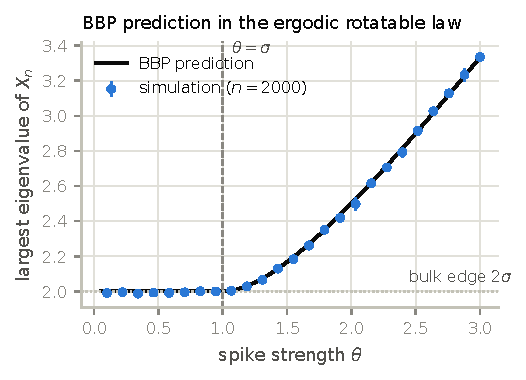
\includegraphics[width=0.55\textwidth]{figures/figS2_bbp_check.pdf}
\caption{Largest eigenvalue of the ergodic law versus spike strength
($n=2000$; mean $\pm$ s.d.\ over 6 replicates) against the prediction
of Proposition~S2; the transition is at $\theta=\sigma$.}
\label{fig:bbpcheck}
\end{figure}

\begin{figure}[h]
\centering
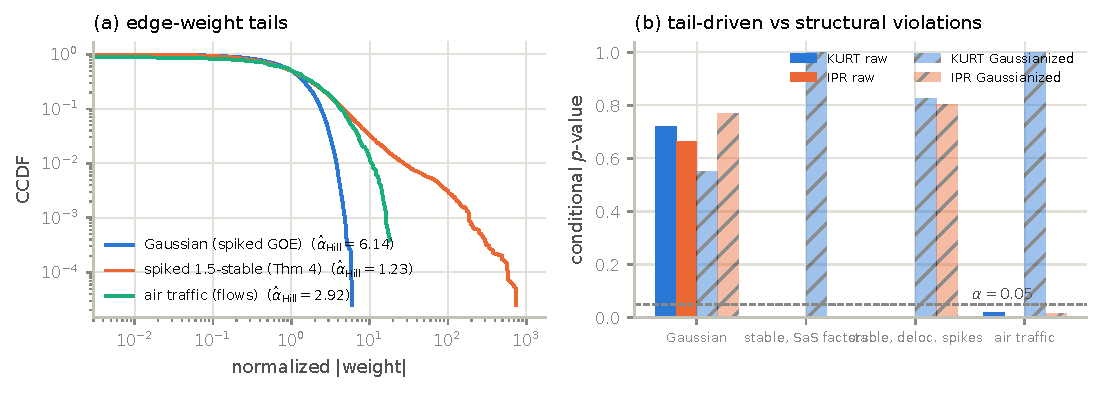
\includegraphics[width=\textwidth]{figures/fig5_heavy.pdf}
\caption{Heavy tails. (a) CCDFs of normalized edge weights with Hill
indices: spiked GOE, the spiked $1.5$-stable law of
Theorem~\ref{thm:stable}, and air traffic. (b) Conditional $p$-values
of kurtosis and IPR, raw and after Gaussianization, for the Gaussian
control, the $\SaS$-factor model, the delocalized-spike control, and
air traffic (first tie seed shown; ranges in Table~\ref{tab:real} and
text).}
\label{fig:heavy}
\end{figure}

\begin{table}[h]
\centering\small
\caption{Rejection rates at nominal $0.05$ of three null models under
the same rotatable truth (spiked GOE, $0$--$3$ random spikes, $n=120$,
$R=100$, $B=99$, hollow pipeline). The Haar-conditional row is the
level study of Figure~2(a) ($R=250$).}
\label{tab:baselines}
\begin{tabular}{lcccccc}
\toprule
Null model & IPR & eigenvector KS & clustering & strength CV & kurtosis & combined\\
\midrule
Haar-conditional (this paper) & \multicolumn{5}{c}{uniform $p$-values (Fig.~2a)} & 0.068\\
Weight permutation & 0.07 & 0.05 & 0.57 & 0.42 & 0.00 & 0.51\\
Fitted-spike parametric bootstrap & 0.02 & 0.07 & 0.10 & 0.03 & 0.06 & 0.03\\
\bottomrule
\end{tabular}
\end{table}

\section{Data, preprocessing, and computation}
\label{supp:data}

\subsection{Data sources}

\emph{Human connectome (HCP group average).} Cortical functional and
structural connectivity matrices distributed with the ENIGMA toolbox
\citep{lariviere2021enigma}, derived from Human Connectome Project young
adult data \citep{vanessen2013wu}: group-average resting-state functional
correlation matrix on the Schaefer 200-parcel cortical parcellation
\citep{schaefer2018local}. Preprocessing: Fisher $z$-transform of
correlations, diagonal set to zero (zero-diagonal completion,
Remark~\ref{rem:hollow}).

\emph{S\&P 500.} Daily closing prices of S\&P~500 constituents,
2013-02-08 to 2018-02-07 (public mirror of the Kaggle S\&P~500 dataset;
the 29\,MB price file is not shipped in the supplement and downloads with
one command documented in \texttt{data/README.md}). Stocks with
incomplete histories dropped; $n=300$ stocks subsampled at random (seed
fixed); log-returns standardized per window; Pearson correlation over
120-trading-day windows advanced by 42 days (28 windows); Fisher $z$;
zero diagonal. Windows overlap in time, and all cross-window regressions
in Section~\ref{sec:exp-cohort} are reported as descriptive for this
reason.

\emph{Air traffic.} U.S.\ airport-pair flight counts (the
\texttt{flights-airport} table of the Vega datasets collection, derived
from U.S.\ DOT/BTS data); flows symmetrized by summing directions,
airports with degree $<5$ removed ($n=183$); tests run on
$\log(1+\mathrm{flow})$; Hill estimator on the upper 5\% of raw positive
flows.

\emph{ABIDE (referenced).} The subject-level replication protocol uses
the ABIDE preprocessed connectomes
\citep{craddock2013neuro,dimartino2014autism} (C-PAC pipeline, CC200
atlas \citep{craddock2012whole}, band-pass filtered, global signal
regressed), which require no data-use agreement. Subject-level ABIDE data were not analyzed for this draft; the
released fetch and analysis scripts specify the intended analysis,
and the cohort analysis of Section~\ref{sec:exp-cohort} uses
synthetic cohorts of
matched dimensions, clearly labeled; the download script
\texttt{fetch\_real\_data.py} reproduces the full pipeline (per-subject
tests, feature construction, classification) on an unrestricted machine.

\subsection{Statistics and testing conventions}

For a hollow symmetric $X$ with eigenpairs $(\mu_j,v_j)$ ordered by
$|\mu_j|$: IPR $=\max_{k\le K_{\mathrm{loc}}}\sum_i V_{ik}^4$ with
$K_{\mathrm{loc}}=10$; eigenvector KS
$=\max_{k\le3}\mathrm{KS}(\sqrt n\,v_k,\,N(0,1))$; weighted clustering
$=$ mean Onnela intensity on the positive part
\citep{onnela2005intensity}; modularity $=$ Newman leading-eigenvector
bipartition value on the positive part \citep{newman2006};
strength CV $=$ coefficient of variation of $\sum_j|X_{ij}|$; kurtosis
$=$ excess kurtosis of off-diagonal entries. Upper-tailed Monte Carlo
$p$-values $(1+\#\{T_b\ge T_{\rm obs}\})/(B+1)$ throughout; lower-tailed
values follow by the formula in Section~\ref{sec:test} and $p$-values
near $1$ are read as lower-tail findings; $B=499$ (HCP), $199$ (air
traffic, diagnostics), $99$ (S\&P windows, level and power simulations,
per-subject cohort tests). Conditional residuals and $z$-scores
(Definition~\ref{def:residual}) are estimated from the same draws.

\emph{Gaussianization and ties.} $G$ maps the off-diagonal entries to
normal scores, scaled by the empirical standard deviation, symmetrically.
Ties, which are widespread for the air-traffic network because most
airport pairs have zero flow, are broken uniformly at random; all
Gaussianized air-traffic analyses are repeated over five tie-breaking
seeds and reported as ranges.

\emph{Cohort protocol (Section~\ref{sec:exp-cohort}).} $S=240$ subjects
per cohort, $n=200$, two groups of 120. Feature sets: spectral (top 10
and bottom 3 eigenvalues plus three spectral moments), non-spectral
summaries (the simulation battery of Section~5, $q=5$), conditional residuals of those
summaries (observed minus Haar-conditional mean given the subject's
spectrum, 32 draws per subject), and spectral plus summaries. Classifier:
$\ell_2$-regularized logistic regression, standardized features,
stratified 5-fold cross-validation, AUC. Per-subject rotatability tests:
$B=99$, Bonferroni over the five statistics at level $0.05$, 20 subjects
per group.

\subsection{Computation and reproducibility}

Haar matrices are generated by QR decomposition of Ginibre matrices with
sign correction; $p$-stable variates by Chambers--Mallows--Stuck. All
figures and tables regenerate from the scripts
\texttt{exp1\_bbp.py}, \texttt{exp2\_test.py},
\texttt{exp2c\_corr\_level.py}, \texttt{exp3\_real.py},
\texttt{exp4\_suff.py}, \texttt{exp5\_heavy.py} (shared library
\texttt{common.py}) with the fixed seed 20260812 (20260813 for residual
features and per-subject tests); total runtime is under one hour on two
CPU cores, and no GPU is used. The complete code, including the
real-data fetch scripts, is provided in the supplement
(\texttt{code/} directory of this project).


\bibliographystyle{apalike}
\bibliography{refs}

\end{document}
